\documentclass[14pt]{memoir}

\usepackage{geometry}
\usepackage[utf8]{inputenc}
\usepackage{amsmath}
\usepackage{amsfonts}
\usepackage{amssymb}
\usepackage{graphicx}
\usepackage[utf8]{inputenc}
\usepackage{amsmath}
\usepackage{amsfonts}
\usepackage{amssymb}
\usepackage[shortlabels]{enumitem}
\usepackage{listings}
\usepackage{xcolor}
\usepackage[most]{tcolorbox}
\usepackage{mathtools}
\usepackage{float}
\usepackage[colorlinks=false, linktocpage=true]{hyperref}

\usepackage{booktabs}% http://ctan.org/pkg/booktabs
\newcommand{\tabitem}{~~\llap{\textbullet}~~}
\usepackage{longtable}
 
\usepackage{caption}
\DeclareCaptionType{code}[Code Listing][List of Code Listings] 

\definecolor{codegreen}{rgb}{0,0.6,0}
\definecolor{codegray}{rgb}{0.5,0.5,0.5}
\definecolor{codepurple}{rgb}{0.58,0,0.82}
\definecolor{backcolour}{rgb}{0.95,0.95,0.92}
 
\lstdefinestyle{mystyle}{
    backgroundcolor=\color{backcolour},   
    commentstyle=\color{codegreen},
    keywordstyle=\color{magenta},
    numberstyle=\tiny\color{codegray},
    stringstyle=\color{codepurple},
    basicstyle=\ttfamily\footnotesize,
    breakatwhitespace=false,         
    breaklines=true,                 
    captionpos=b,                    
    keepspaces=true,                 
    numbers=left,                    
    numbersep=5pt,                  
    showspaces=false,                
    showstringspaces=false,
    showtabs=false,                  
    tabsize=2
}
 
\lstset{style=mystyle}

\setlength{\parindent}{0em}
\setlength{\parskip}{1em}

\author{Brian Rashap, Ph.D.}
\title{PHYS 1320 - Calculus-based Physics II}

\geometry{letterpaper, portrait, margin=0.75in}

\begin{document}
\frontmatter

\maketitle


\mainmatter

\chapter{Module 1: Chapter 5 - Electric Charges and Fields}

From Newton's Second Laws of Mechanics:

\begin{equation}
F = ma
\end{equation}

A force can be recognized by the effect it has on an object. When studying gravitation, we examined the force of gravity that acts on all objects with mass. Similarly, the electric force acts on all objects with a property called charge. While gravity is an attractive force, the electric force can be either attractive or repulsive.  

\section{Section 5.1 Electric Charge}

The ancient Greek philosopher Thales of Miletus (624-546 BCE)recorded that when amber was vigorously rubbed with a piece of fur, it created a force that attracted them to each other. They also attracted other non-metallic objects even when not touched. 

\begin{figure}[h]
\begin{center}
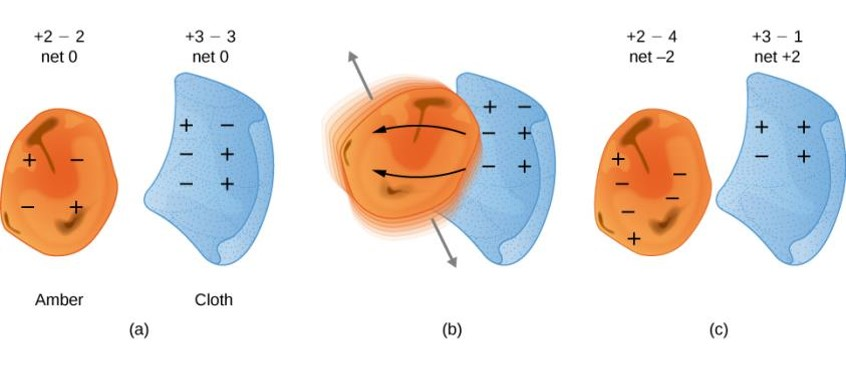
\includegraphics[scale=0.40]{fig/fig_05_05.jpg}
\caption{Materials rubbed together}
\label{fig:05_05}
\end{center}
\end{figure}

The English physicist William Gilbert (1544-1603) also studied attractive forces. He worked with a variety of substances. His findings included:
\begin{itemize}
\item Metals never exhibited this force, whereas minerals did
\item Two "electrified" amber rods would repel each other. 
\end{itemize}

This suggested that were two types of electric properties: attractive and repulsive. This property came to be known as Electric Charge. The force is repulsive between between the same type of charge and attractive between the charges are of opposite types. Named after French physicist Charles Augustine de Coulomb (1736-1806), the unit of electric charge is the coulomb (C).

The American statesman and scientist Benjamin Franklin found that he could concentrate charge in Leyden jar \footnote{Its invention was a discovery made independently by German cleric Ewald Georg von Kleist on 11 October 1745 and by Dutch scientist Pieter van Musschenbroek of Leiden (Leyden), Netherlands in 1745–1746. The invention was named after the city.} (a glass jar with two metal sheets one on the inside and one on the outside (essentially what we now call a capacitor). Franklin pointed out that the behavior could be explained by one type of charge remaining motionless and the other charge flowing from one piece of foil to the other. He had no way of determining which type of charge was moving, and unfortunately he guessed wrong: it was since learned that the charges that flow are the ones that Franklin named "negative" and the "positive" charges remain motionless.

\begin{figure}[h]
\begin{center}
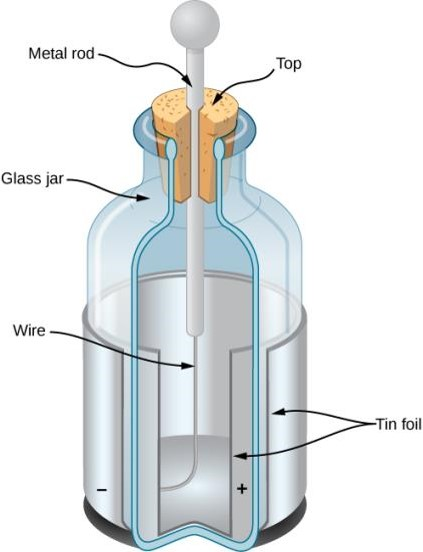
\includegraphics[scale=0.40]{fig/fig_05_06.jpg}
\caption{Leyden Jar}
\label{fig:05_06}
\end{center}
\end{figure}

Observations about the Electric Force:
\begin{itemize}
\item The force acts without physical contact between objects
\item The force is attractive or repulsive
\item Not all objects are affected by this force
\item The magnitude of the force decreases rapidly with distance between objects
\end{itemize}

Properties of Electric Charge
\begin{itemize}
\item Charge is quantized - The smallest amount of charge an object can have is $e = 1.602 * 10^{-19} C$. The charge on any object must be an integer multiple of $e$.
\item The magnitude of a change is independent of the type. The smallest positive charge is $1.602 * 10^{-19} C$ and the smallest negative charge is $-1.602 * 10^{-19} C$; these values are exactly equal in magnitude. 
\item Charge is conserved. Change can not be created or destroyed. It can only be transferred. The net charge of the universe is constant. 
\item Charge is conserved in a closed system. Total charge in a closed system remains constant.
\end{itemize}
These last two items are referred to as the Law of Conservation of Charge. 

\subsection{The Sources of Charge: The Structure of the Atom}

Atomic structure terminology
\begin{itemize}
\item Electron
\item Proton
\item Neutron
\item Ion
\end{itemize}

This simplified model of a hydrogen atom shows a positively charged nucleus (consisting, in the case of hydrogen, of a single proton), surrounded by an electron “cloud.” The charge of the electron cloud is equal (and opposite in sign) to the charge of the nucleus, but the electron does not have a definite location in space;  hence, its representation here is as a cloud. Normal macroscopic amounts of matter contain immense numbers of atoms and molecules, and, hence, even greater numbers of individual negative and positive charges. 

\begin{figure}[h]
\begin{center}
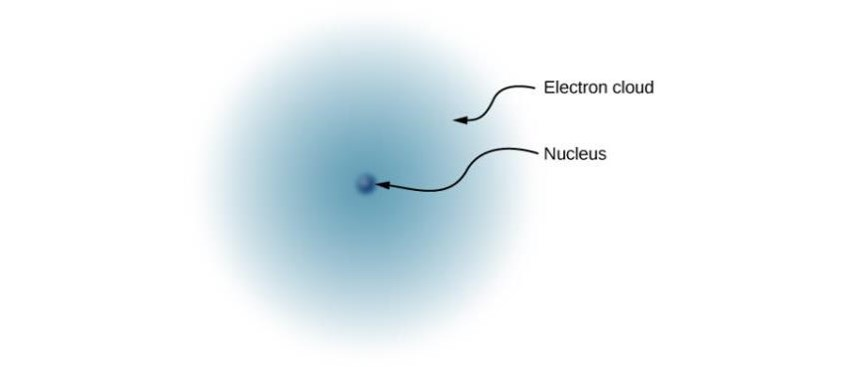
\includegraphics[scale=0.40]{fig/fig_05_07.jpg}
\caption{Simplified model of a hydrogen atom}
\label{fig:05_07}
\end{center}
\end{figure}

The nucleus of a carbon atom is composed of six protons and six neutrons. As in hydrogen, the surrounding six electrons do not have definite locations and so can be considered to be a sort of cloud surrounding the nucleus.


\begin{figure}[h]
\begin{center}
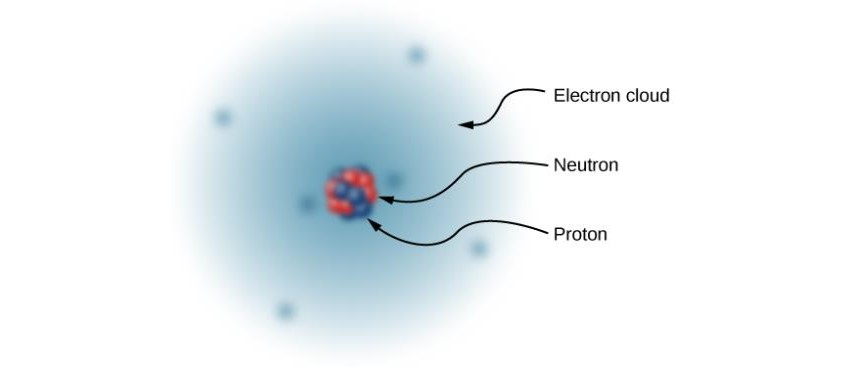
\includegraphics[scale=0.40]{fig/fig_05_08.jpg}
\caption{Carbon atom}
\label{fig:05_08}
\end{center}
\end{figure}

\section{Conductors, Insulators, and Charging by Induction}

\subsection{Conductors}

Electrons surround the tiny nucleus in the form of a (comparatively) vast cloud of negative charge. However, this cloud does have a definite structure to it. If we consider an atom of copper, there is an outermost electron that is only loosely bound to the atom’s nucleus. It can be easily dislodged; it then moves to a neighboring atom. In a large mass of copper atoms (such as a copper wire or a sheet of copper), these vast numbers of outermost electrons (one per atom) wander from atom to atom, and are the electrons that do the moving when electricity flows. These wandering, or “free,” electrons are called conduction electrons, and copper is therefore an excellent conductor (of electric charge). All conducting elements have a similar arrangement of their electrons, with one or two conduction electrons. This includes most metals.

\subsection{Insulators}

Insulators, in contrast, are made from materials that lack conduction electrons; charge flows only with great difficulty, if at all. Even if excess charge is added to an insulating material, it cannot move, remaining indefinitely in place. This is why insulating materials exhibit the electrical attraction and repulsion forces described earlier, whereas conductors do not; any excess charge placed on a conductor would instantly flow away (due to mutual repulsion from existing charges), leaving no excess charge around to create forces. Charge cannot flow along or through an insulator, so its electric forces remain for long periods of time. (Charge will dissipate from an insulator, given enough time.) As it happens, amber, fur, and most semi-precious gems are insulators, as are materials like wood, glass, and plastic.

\subsection{Charging by Induction}

Induced polarization: A positively charged glass rod is brought near the left side of the conducting sphere, attracting negative charge and leaving the other side of the sphere positively charged. Although the sphere is overall still electrically neutral, it now has a charge distribution, so it can exert an electric force on other nearby charges. Furthermore, the distribution is such that it will be attracted to the glass rod.


\begin{figure}[h]
\begin{center}
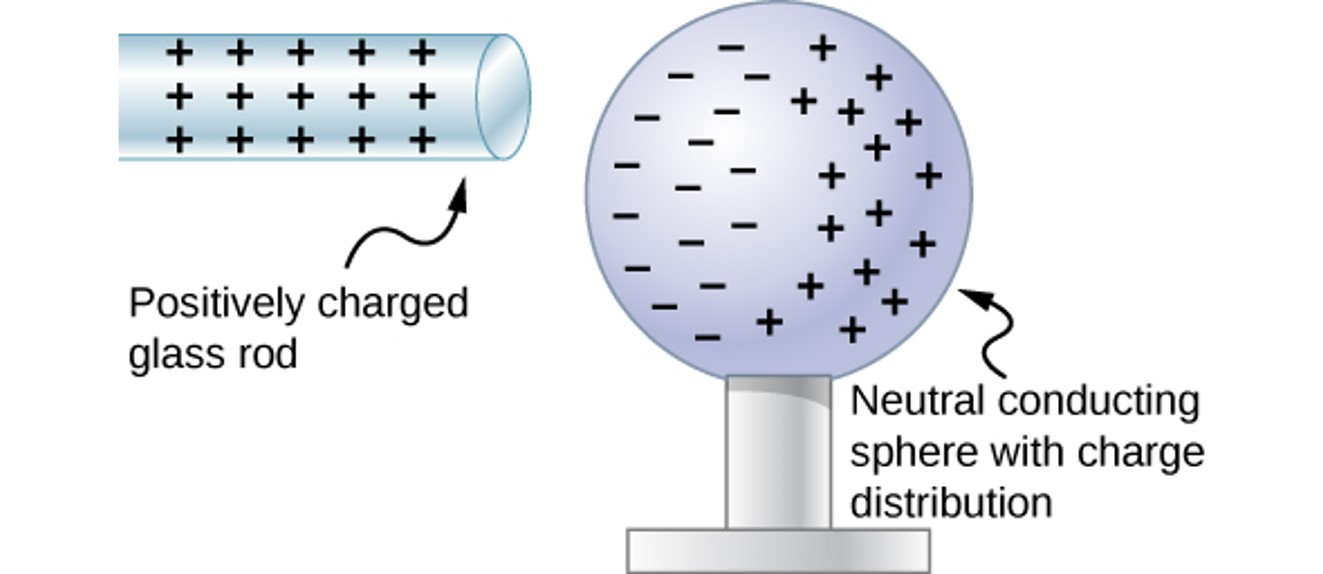
\includegraphics[scale=0.40]{fig/fig_05_10.jpg}
\caption{Induced Polarization}
\label{fig:05_10}
\end{center}
\end{figure}

Both positive and negative objects attract a neutral object by polarizing its molecules.
\begin{itemize}
\item A positive object brought near a neutral insulator polarizes its molecules. There is a slight shift in the distribution of the electrons orbiting the molecule, with unlike charges being brought nearer and like charges moved away. Since the electrostatic force decreases with distance, there is a net attraction.
\item  A negative object produces the opposite polarization, but again attracts the neutral object. 
\item The same effect occurs for a conductor; since the unlike charges are closer, there is a net attraction.
\end{itemize}

\begin{figure}[h]
\begin{center}
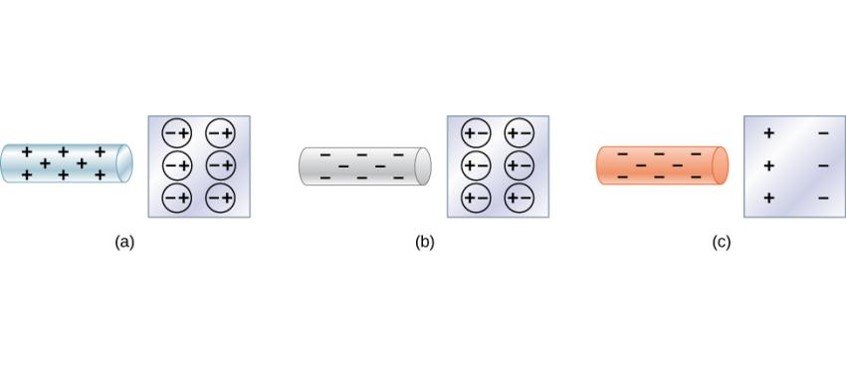
\includegraphics[scale=0.60]{fig/fig_05_11.jpg}
\caption{Attraction to neutral objects}
\label{fig:05_11}
\end{center}
\end{figure}

Charging by induction.
\begin{itemize}
\item Two uncharged or neutral metal spheres are in contact with each other but insulated from the rest of the world.
\item A positively charged glass rod is brought near the sphere on the left, attracting negative charge and leaving the other sphere positively charged.
\item The spheres are separated before the rod is removed, thus separating negative and positive charges.
\item The spheres retain net charges after the inducing rod is removed—without ever having been touched by a charged object.
\end{itemize}

\begin{figure}[h]
\begin{center}
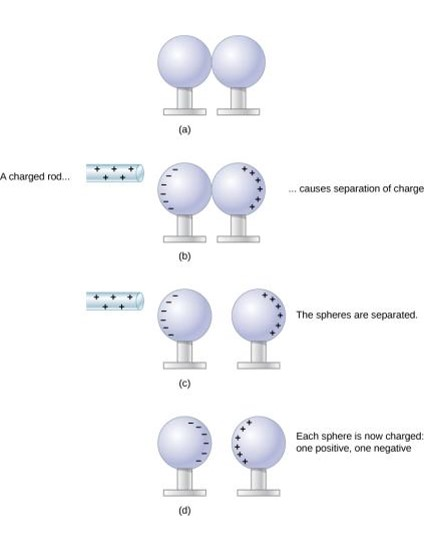
\includegraphics[scale=0.60]{fig/fig_05_12.jpg}
\caption{Charge by Induction}
\label{fig:05_12}
\end{center}
\end{figure}

Similarly using a ground connection

\begin{figure}[H]
\begin{center}
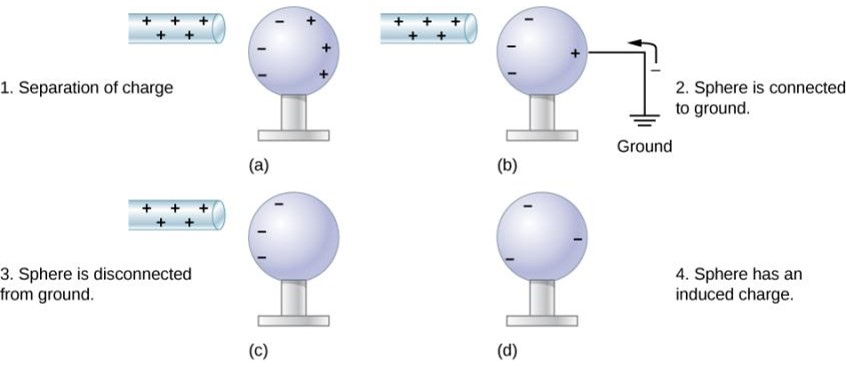
\includegraphics[scale=0.60]{fig/fig_05_13.jpg}
\caption{Charge by Induction with Ground Connection}
\label{fig:05_13}
\end{center}
\end{figure}

\section{Coulombs Law}

Recall from Physics I the gravitational force equation

\begin{figure}[h]
\begin{center}
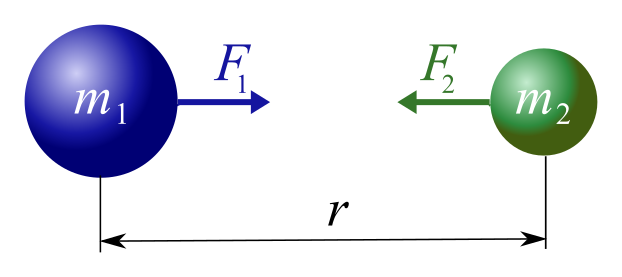
\includegraphics[scale=0.60]{fig/NewtonsLawGravitation.png}
\caption{Newtons Law Gravitation}
\label{fig:NLG}
\end{center}
\end{figure}

\begin{equation}
F_G = G \frac{m_1 m_2}{r^{2}}
\end{equation}



For the electric force, let
\begin{itemize}
\item $q_1, q_2 = $ the net electric charges of two objects
\item $\vec{r}_{12} = $ the vector displacement from $q_1$ to $q_2$.
\end{itemize}

\begin{equation}
F \propto \frac{q_1 q_2}{r^{2}_{12}}
\end{equation}

\begin{figure}[h]
\begin{center}
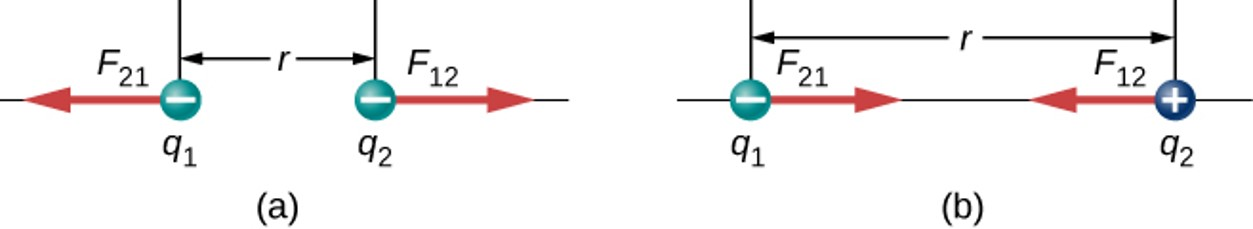
\includegraphics[scale=0.60]{fig/fig_05_14.jpg}
\caption{Electrostatic Force}
\label{fig:05_14}
\end{center}
\end{figure}

Coulomb's Law: the electric force between two electrically charged particles is given by

\begin{equation}
\vec{F} = \frac{1}{4 \pi \epsilon_0} \frac{q_1 q_2}{r^{2}_{12}} \hat{r}_{12}
\end{equation}

where $\vec{r}_{12}$ is the unit vector from particle 1 to particle 2, and 
where $\epsilon_0$ is the permittivity of free space

\begin{equation}
\epsilon_0 = 8.85 * 10^{-12} \frac{C^2}{N \cdot m^2}
\end{equation}

Which leads to Coulomb's constant ($k$):

\begin{equation}
k = \frac{1}{4 \pi \epsilon_0} = 8.99 * 10^9 \frac{N \cdot m^2}{C^2} 
\end{equation}


\subsection{Example: Force on the Electron in a Hydrogen Atom}

Proton has a positive charge of $+e$, and an electron has a negative charge of $-e$. In the "ground state" of the atom, the electron orbits the proton at a probably distance of $5.29 * 10^{-11} m$.

\begin{equation}
q_1 = +e = +1.602 * 10^{-19} C 
\end{equation}

\begin{equation}
q_2 = -e = -1.602 * 10^{-19} C 
\end{equation}

\begin{equation}
r = 5.29 * 10^{-11} m
\end{equation}

The magnitude of the force

\begin{equation}
F = \frac{1}{4 \pi \epsilon_0} \frac{\lvert e \lvert^2}{r^{2}} = 8.99 * 10^9 \frac{N \cdot m^2}{C^2} * \frac{(1.602 * 10^{-19} C)^2}{(5.29 * 10^{-11} m)^2} = 8.25 * 10^{-8} N
\end{equation}

The force is thus expressed as

\begin{equation}
\vec{F} = (8.25 * 10^{-8} N) \hat{r}
\end{equation}

\subsection{Multiple Sources of Charge}

As with the forces encountered in Physics I, the net electric force is the vector sum of the individual forces. 

\begin{equation}
\vec{F}(r) = \frac{1}{4 \pi \epsilon_0} Q \sum_{i=1}^{N}\frac{q_i}{r_i^2}\hat{r}_i
\end{equation}

where $Q$ represents the charge of a particle that experiences the force $\vec{F}$ and is located at $\vec{r}$ from the origin; $q_i$ are the N source charges, and the vectors $\vec{r}_i = r_i \hat{r}_i$ are the displacements from the position of the ith charge to the position of Q. All of this is with the simplifying assumption that the source charges are all fixed in place somehow. This is referred to as the electrostatic force. 

\begin{figure}[h]
\begin{center}
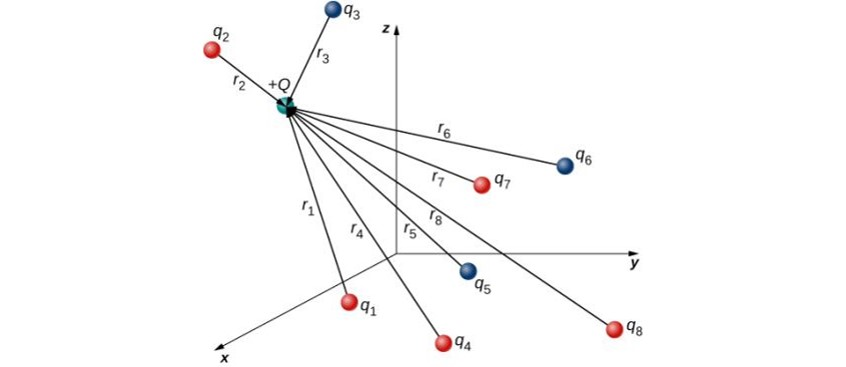
\includegraphics[scale=0.60]{fig/fig_05_15.jpg}
\caption{Multiple Source Charges}
\label{fig:05_15}
\end{center}
\end{figure}


insert example 5.2

\section{Electric Field}

Next we define the Electric Field, which is independent of the test charge Q, and only depends on the configuration of the source charges. 

\begin{equation}
\vec{F} = Q \cdot \vec{E}
\end{equation}

where 

\begin{equation}
\vec{E}(P) = \frac{1}{4 \pi \epsilon_0} \sum_{i=1}^{N}\frac{q_i}{r_i^2}\hat{r}_i
\end{equation}

expresses the Electric Field at position $P = P(x,y,z)$ of the N source charges. 

\begin{figure}[h]
\begin{center}
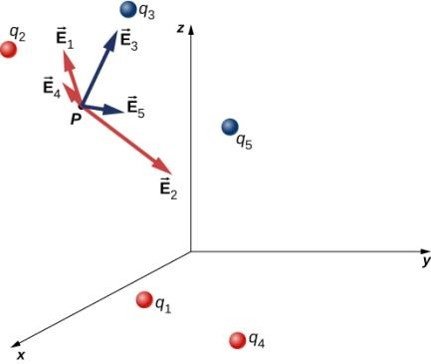
\includegraphics[scale=0.60]{fig/fig_05_18.jpg}
\caption{Electric Field - Multiple Source Charges}
\label{fig:05_18}
\end{center}
\end{figure}


This is analogous to the graviational field $\vec{g}$ of the Earth

\begin{equation}
\vec{g} = G \frac{M}{r^2}\hat{r}
\end{equation}

which gives us $9.81 \frac{m}{s}$ near the Earth's surface.


The Electric Field is
\begin{itemize}
\item A vector field
\item Obeys superposition
\item By convention, the Electric Field points away from the positive charge. 
\end{itemize}

\section{Calculating Electric Field Charge Distributions}

\begin{figure}[h]
\begin{center}
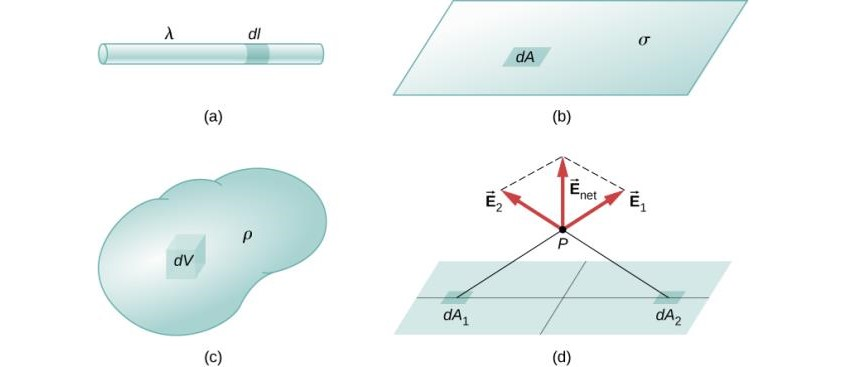
\includegraphics[scale=0.60]{fig/fig_05_22.jpg}
\caption{Configuration of Charge}
\label{fig:05_22}
\end{center}
\end{figure}

Definitions of charge density
\begin{itemize}
\item $\lambda \equiv $ charge per unit length (linear charge density) in $\frac{C}{m}$
\item $\sigma \equiv $ charge per unit area (surface charge density) in $\frac{C}{m^2}$
\item $\rho \equiv $ charge per unit volume (volume charge density) in $\frac{C}{m^3}$
\end{itemize}

Given these densities, the differential charge ($dq$) becomes $\lambda dl$, $\sigma dA$, and $\rho dV$, respectively. 

For these distributions, the summation becomes an integral
\begin{itemize}
\item Point Charge
	\begin{equation}
	\vec{E}(P) = \frac{1}{4 \pi \epsilon_0} \sum_{i=1}^{N}\frac{q_i}{r^2}\hat{r}
	\end{equation}
\item Line Charge
	\begin{equation}
	\vec{E}(P) = \frac{1}{4 \pi \epsilon_0} \int_{line}(\frac{\lambda dl}{r^2})\hat{r}
	\end{equation}
\item Surface Charge
	\begin{equation}
	\vec{E}(P) = \frac{1}{4 \pi \epsilon_0} \int_{surface}(\frac{\sigma dA}{r^2})\hat{r}
	\end{equation}
\item Volume Charge
	\begin{equation}
	\vec{E}(P) = \frac{1}{4 \pi \epsilon_0} \int_{volume}(\frac{\rho dV}{r^2})\hat{r}
	\end{equation}
	
\end{itemize}

As $P = P(x,y,z)$, the integral is shorthand for three integrals (one in each direction)

\begin{equation}
\vec{E}_x(P) = \frac{1}{4 \pi \epsilon_0} \int_{line}(\frac{\lambda dl}{r^2})_x,
\vec{E}_y(P) = \frac{1}{4 \pi \epsilon_0} \int_{line}(\frac{\lambda dl}{r^2})_y,
\vec{E}_z(P) = \frac{1}{4 \pi \epsilon_0} \int_{line}(\frac{\lambda dl}{r^2})_z
\end{equation}


\subsection{Electric Field of a Line Segment}

\begin{figure}[h]
\begin{center}
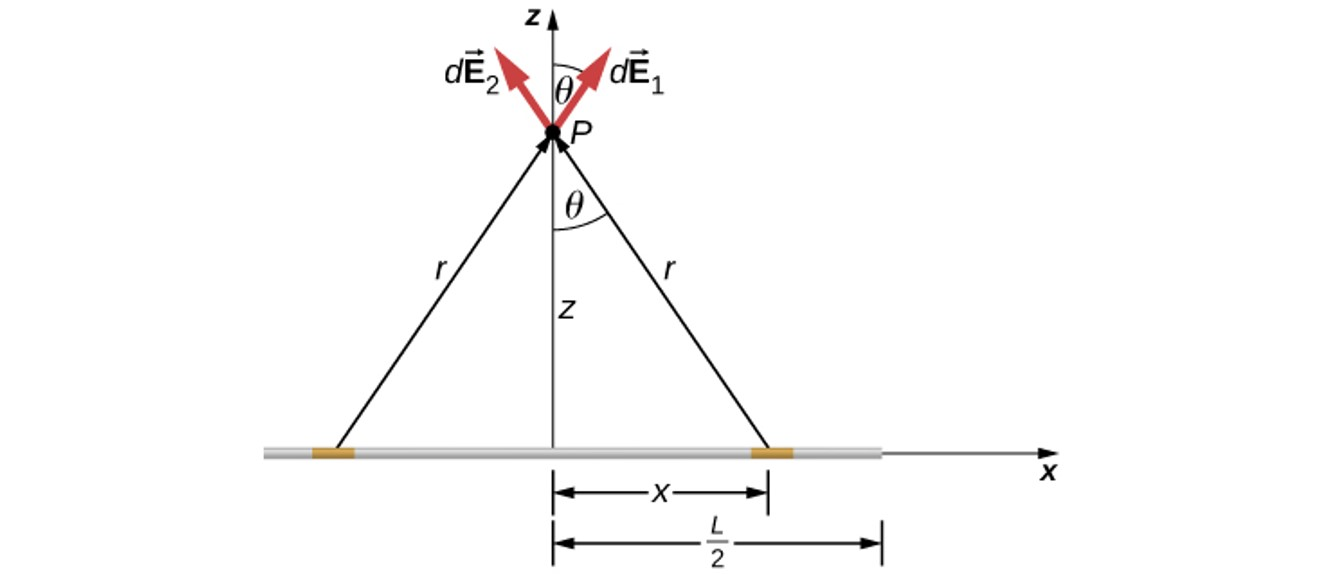
\includegraphics[scale=0.60]{fig/fig_05_23.jpg}
\caption{A uniformly charged segment of wire. The electric field at point P can be found by applying the superposition principle to symmetrically placed charge elements and integrating.
}
\label{fig:05_23}
\end{center}
\end{figure}


Start with 

\begin{equation}
\vec{E}(P) = \frac{1}{4 \pi \epsilon_0} \int_{line}(\frac{\lambda dl}{r^2})\hat{r}
\label{Eline}
\end{equation}
	
The symmetry of the arrangement implies the horizontal components cancel.

\begin{equation}
\vec{E}(P) = \vec{E_1} + \vec{E_2} = E_{1,x} \hat{i} + E_{1,z} \hat{k} + E_{2,x} (-\hat{i}) + E_{2,z} \hat{k}
\end{equation}

Due to symmetry, $E_{1,x} = E_{2,x}$, and as their directions are opposite, they cancel. So,

\begin{equation}
\vec{E}(P) = E_{1,z} \hat{k}  + E_{2,z} \hat{k} = E_1 \cos{\theta} \hat{k} + E_2 \cos{\theta} \hat{k}
\end{equation}

As these components are also equal, substituting into Equation \ref{Eline} yields:

\begin{equation}
\vec{E}(P) = \frac{1}{4 \pi \epsilon_0} \int_{0}^{\frac{L}{2}}(\frac{2 \lambda dx}{r^2} \cos{\theta})\hat{k}
\end{equation}

To calculate the integral, we note that 

\begin{equation}
r = \sqrt{(x^2 + z ^2)}
\end{equation}

and

\begin{equation}
\cos{\theta} = \frac{z}{r} = \frac{z}{\sqrt{(x^2 + z ^2)}} =  \frac{z}{(x^2 + z ^2)^{\frac{1}{2}}}
\end{equation}

Substituting for $\cos{\theta}$:

\begin{equation}
\vec{E}(P) = \frac{1}{4 \pi \epsilon_0} \int_{0}^{\frac{L}{2}}(\frac{2 \lambda dx}{(x^2 + z ^2)} \frac{z}{(x^2 + z ^2)^{\frac{1}{2}}})\hat{k}
\end{equation}

\begin{equation}
\vec{E}(P) = \frac{1}{4 \pi \epsilon_0} \int_{0}^{\frac{L}{2}}(\frac{2 \lambda z}{(x^2 + z ^2)^{\frac{3}{2}}}) dx \hat{k}
\end{equation}

Integrating utilizing Trig Substitution (See Appendix \ref{sec:trigsub}):
\begin{equation}
\vec{E}(P) = \frac{2 \lambda z}{4 \pi \epsilon_0} [\frac{x}{z^2 \sqrt{(x^2 + z ^2)}}]\bigg\rvert_{0}^{\frac{L}{2}} \hat{k}
\end{equation}

or

\begin{equation}
\vec{E}(z) = \frac{1}{4 \pi \epsilon_0} \frac{\lambda L}{z \sqrt{(\frac{L}{4} + z^2)}} \hat{k}
\end{equation}

For an infinite line: $L = \infty$

\begin{equation}
\vec{E}(z) = \frac{1}{4 \pi \epsilon_0} \frac{2 \lambda}{z} \hat{k}
\end{equation}

noting that we lost the $\frac{1}{r^2}$ dependence

For a finite line of charge with $z >> L$

\begin{equation}
\vec{E}(z) = \frac{1}{4 \pi \epsilon_0} \frac{\lambda L}{z^2} \hat{k}
\end{equation}

Recalling that $q = \lambda L$, then we get the expression of the field of a point charge.



\section{Electric Field Lines}

Electric Field Lines allow us to visualize the electric field in space

\begin{figure}[H]
\begin{center}
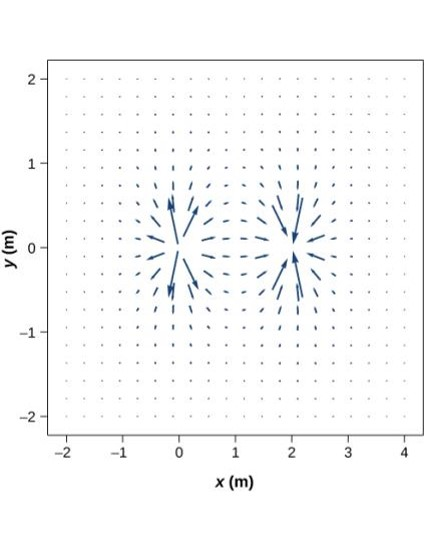
\includegraphics[scale=0.60]{fig/fig_05_28.jpg}
\caption{Vector field of dipole}
\label{fig:05_28}
\end{center}
\end{figure}

Electric Field Line "Rules"

\begin{itemize}
\item Either begin at a positive charge or come in from infinity
\item Either end at a negative charge or extend out to infinity
\item The number of lines originating or terminating is proportional to the amount of charge.
\item The density at any point in space is proportional to (and therefore is representative of) the magnitude of the field at that point in space 
\item The field lines never cross
\end{itemize}

\begin{figure}[h]
\begin{center}
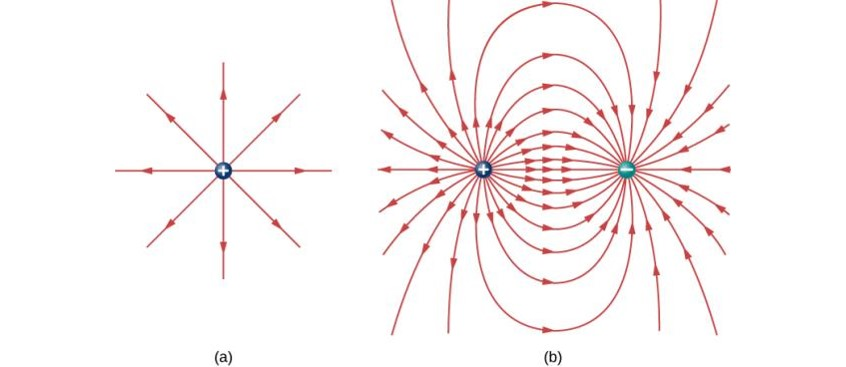
\includegraphics[scale=0.60]{fig/fig_05_29.jpg}
\caption{Electric Field of a dipole}
\label{fig:05_29}
\end{center}
\end{figure}

\begin{figure}[h]
\begin{center}
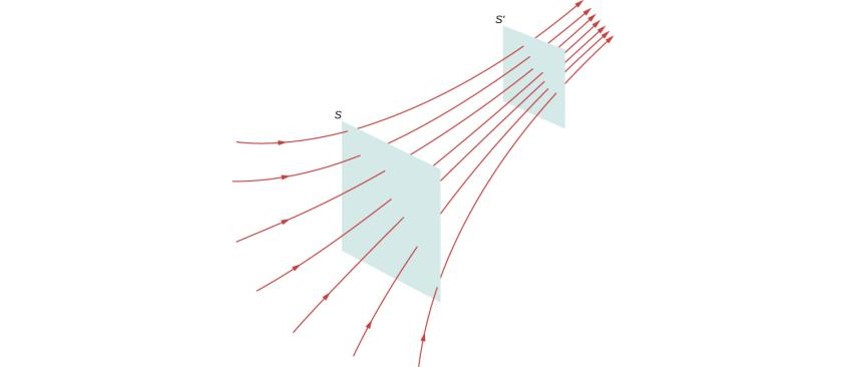
\includegraphics[scale=0.60]{fig/fig_05_30.jpg}
\caption{Field Line Density}
\label{fig:05_30}
\end{center}
\end{figure}

\begin{figure}[h]
\begin{center}
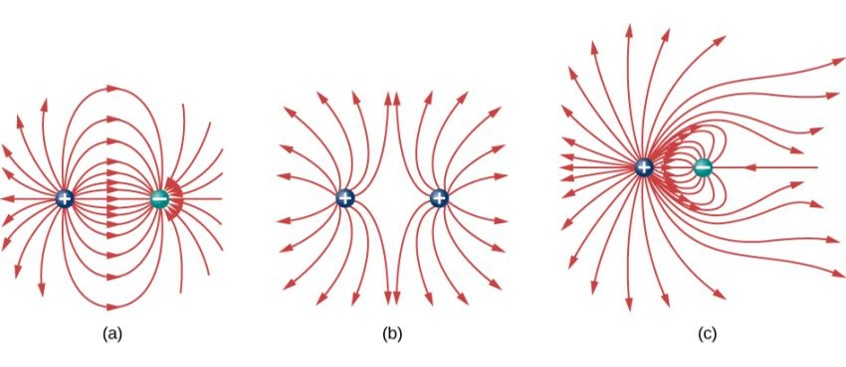
\includegraphics[scale=0.60]{fig/fig_05_31.jpg}
\caption{Typical Diagrams}
\label{fig:05_31}
\end{center}
\end{figure}

\chapter{Module 2: Chapter 6 - Gauss's Law}

Four main topics:

\begin{itemize}
\item Electric Flux
\item Guass's Law
\item Calculating Electric Field with Guass's Law
\item Electric Field inside Conductors
\end{itemize}


\section{Electric Flux}

Flux describes how much of something goes through a given area. More formally, flux is the dot-product of a vector field (in our case, the electric field) with an area.  

\begin{figure}[h]
\begin{center}
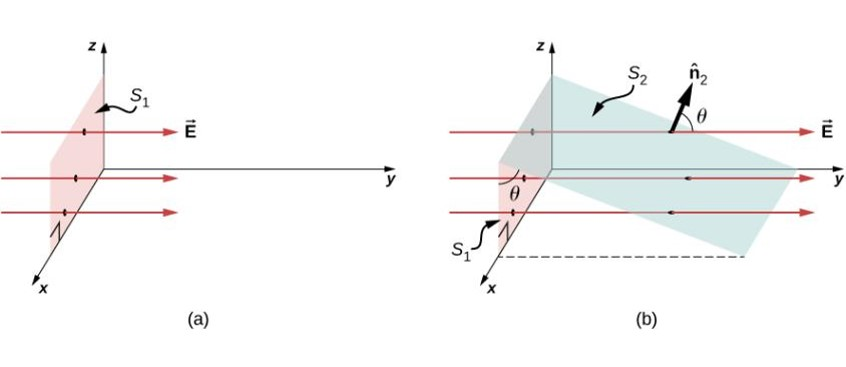
\includegraphics[scale=0.60]{fig/fig_06_04.jpg}
\caption{Flux through a plane}
\label{fig:06_04}
\end{center}
\end{figure}

\subsection{Electric Flux}

For uniform field $\vec{E}$ and a flat surface:
\begin{equation}
\Phi = \vec{E} \cdot \vec{A}
\end{equation}
\begin{equation}
\Phi = E A \cos{\theta}
\end{equation}


\begin{figure}[H]
\begin{center}
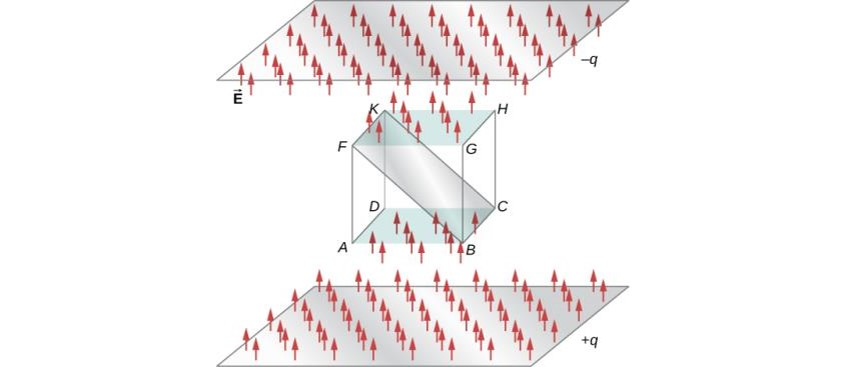
\includegraphics[scale=0.60]{fig/fig_06_07.jpg}
\caption{Flux through a cube}
\label{fig:06_07}
\end{center}
\end{figure}

\begin{itemize}
\item Source and termination of electric field lines are outside the cube
\item There is no charge inside the cube
\item All electric field lines that enter the cube exit it, so the net flux through the cube is zero.
\item By convention: if field lines are leaving a closed surface then $\Phi$ is positive. 
\item For field lines entering a closed surface, $\Phi$ is negative.
\end{itemize}

For a non-flat surface, we can take small patches that approximate a flat surface

\begin{figure}[H]
\begin{center}
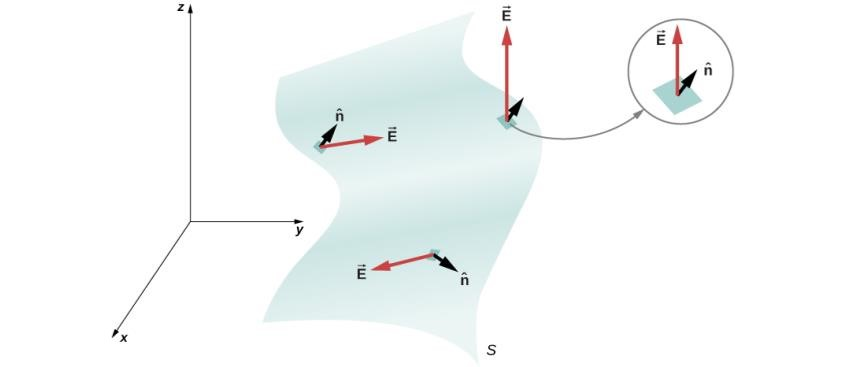
\includegraphics[scale=0.60]{fig/fig_06_08.jpg}
\caption{Surface divided into patches to find flux}
\label{fig:06_08}
\end{center}
\end{figure}

Consider $\vec{E}_i$ to be the electric field over the $i^{th}$ patch ($\delta A_i$), then

\begin{equation}
\Phi_i = \vec{E}_i \cdot \delta \vec{A}_i
\end{equation}

then

\begin{equation}
\Phi = \sum_{i=1}^{N} \Phi_i = \sum_{i=1}^{N} \vec{E}_i \cdot \delta \vec{A}_i
\end{equation}

As the patch gets infinitesimally small, 

\begin{equation}
\delta \vec{A} \rightarrow \hat{n} dA
\end{equation}

and the $\sum$ become an $\int_s$ over the entire surface

For an Open Surface:

\begin{equation}
\Phi = \int_s \vec{E} \cdot \hat{n} dA = \int_s \vec{E}  \cdot d\vec{A}
\end{equation}

For an Closed Surface:

\begin{equation}
\Phi = \oint_s \vec{E} \cdot \hat{n} dA = \oint_s \vec{E}  \cdot d\vec{A}
\label{eq:flux}
\end{equation}

\section{Gauss's Law}

Let's calculate the electric flux through a sphere that surrounds a point charge $q$.

Recall at Point $P$
\begin{equation}
\vec{E}_P = \frac{1}{4 \pi \epsilon_0} \frac{q}{r^2} \hat{r}
\end{equation}

where $\hat{r}$ is the radial unit vector charge at the center to Point $P$.

\begin{figure}[H]
\begin{center}
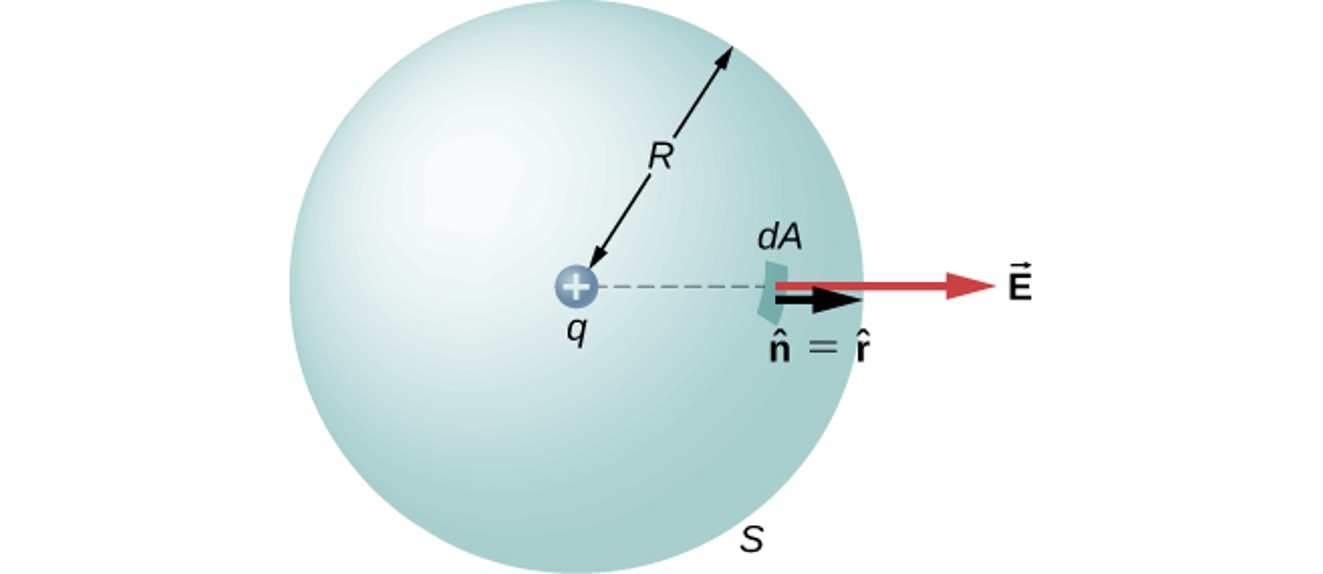
\includegraphics[scale=0.40]{fig/fig_06_13.jpg}
\caption{Closed sphere around point charge P}
\label{fig:06_13}
\end{center}
\end{figure}

Applying the flux equation \ref{eq:flux}, where $\hat{n} = \hat{r}$ and $r = R$, for infinitesimal area $dA$:

\begin{equation}
d\Phi = \vec{E} \cdot \hat{n} dA = \frac{1}{4 \pi \epsilon_0} \frac{q}{R^2} \hat{r} \cdot \hat{r} dA =  \frac{1}{4 \pi \epsilon_0} \frac{q}{R^2} dA
\end{equation}

Integrating

\begin{equation}
\Phi = \frac{1}{4 \pi \epsilon_0} \frac{q}{R^2} \oint_s dA =  \frac{1}{4 \pi \epsilon_0} \frac{q}{R^2} (4 \pi R^2) = \frac{q}{\epsilon_0}
\end{equation}

As r increases, there is a  $\frac{1}{r^2}$ decrease in electric field counteracts the $r^2$ increase in the surface of the sphere and we find that $\Phi = \frac{q}{\epsilon_0}$ is independent of the size of the sphere. 


Gauss's Law
\begin{equation}
\boxed{\Phi_{closedsurface} = \frac{q_{enc}}{\epsilon_0}}
\end{equation}

where $q_{enc}$ is the net charge enclosed by the surface

\section{Applying Gauss's Law}

\subsubsection{Charge Distribution with Spherical Symmetry}

Charge distribution is considered spherically symmetric if the density of charge depends only on the distance from a point in space and not direction. A spherically symmetric charge distribution does not change of you rotate the sphere.

\begin{equation}
\rho(r,\theta,\phi) = \rho(r)
\end{equation}

For spherically symmetric:

\begin{equation}
\vec{E}_P = E_P(r)\hat{r}
\end{equation}

The magnitude of the electric field $\vec{E}$ is the same everywhere on a spherical Gaussian surface concentric with the distribution. For a sphere of radius $r$:

\begin{equation}
\Phi = E_P 4 \pi r^2
\end{equation}

From Gauss's Law
\begin{equation}
4 \pi r^2 E = \frac{q_{enc}}{\epsilon_0}
\end{equation}

Combining, the magnitude $E(r)$ is given by
\begin{equation}
E(r) = \frac{1}{4 \pi \epsilon_0}\frac{q_{enc}}{r^2}
\end{equation}

For a sphere of radius $R$

\begin{equation}
  q_{enc}=\begin{cases}
    q_{tot}, & \text{if } r \geq R.\\
    q_{(r<R)}, & \text{if } r < R.
  \end{cases}
\end{equation}

Which leads to an Electric Field at point P ($E_{out}$ for P outside the sphere, and $E_{in}$ for P inside the sphere

\begin{figure}[H]
\begin{center}
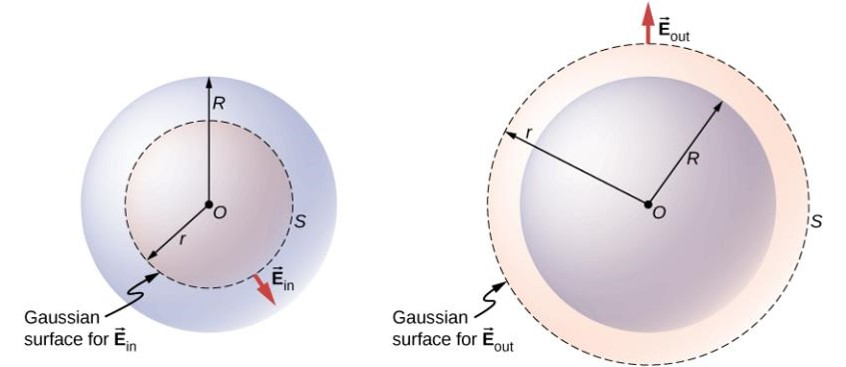
\includegraphics[scale=0.60]{fig/fig_06_23.jpg}
\caption{Outside and inside the sphere}
\label{fig:06_23}
\end{center}
\end{figure}

\begin{equation}
E_{out} = \frac{1}{4 \pi \epsilon_0}\frac{q_{tot}}{r^2}
\end{equation}

\begin{equation}
E_{in} = \frac{1}{4 \pi \epsilon_0}\frac{q_{(r<R)}}{r^2}
\end{equation}

So, what is $q_{enc}$ inside the sphere. Let's assume uniform distribution of charge $\rho_o$

\begin{equation}
q_{enc} = \int \rho_0 dV = \int_{0}^{r} \rho_0 4 \pi r^{\prime} dr^{\prime} = \rho_0 (\frac{4}{3} \pi r^3)
\end{equation}

Therefore

\begin{equation}
E_{out} = \frac{1}{4 \pi \epsilon_0}\frac{q_{tot}}{r^2}, \text{ with: } q_{tot} = \frac{4}{3} \pi R^3 \rho_0
\end{equation}

\begin{equation}
E_{in} = \frac{1}{4 \pi \epsilon_0}\frac{q_{(r<R)}}{r^2} = \frac{\rho_0 r}{3 \epsilon_0}, \text{  since: } q_{(r<R)} = \frac{4}{3} \pi r^3 \rho_0
\end{equation}

\begin{figure}[H]
\begin{center}
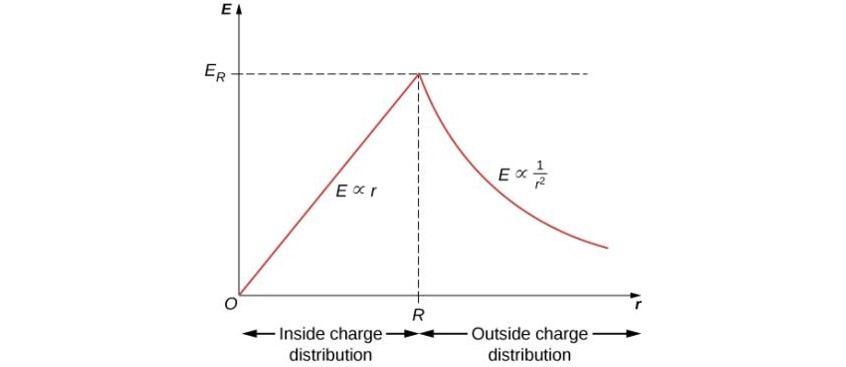
\includegraphics[scale=0.40]{fig/fig_06_24.jpg}
\caption{Electric Field of uniformly charged non-conducting sphere}
\label{fig:06_24}
\end{center}
\end{figure}

\subsubsection{Charge Distribution with Symmetric Cylinder}

Charge distribution is considered cylindrical symmetric if the density of charge depends only on the distance $r$ from the axis, and does not vary along or with direction of axis.

Consider an "infinitely\footnote{In the real world, cylinders are not finite, but if the length $L >> r$ then it can be approximated as infinitely long} long" cylinder with cylindrical symmetric charge distribution.

\begin{equation}
\rho(r,\theta,z) = \rho(r)
\end{equation}

\begin{equation}
\vec{E}_P = E_P(r)\hat{r}
\end{equation}


\begin{figure}[H]
\begin{center}
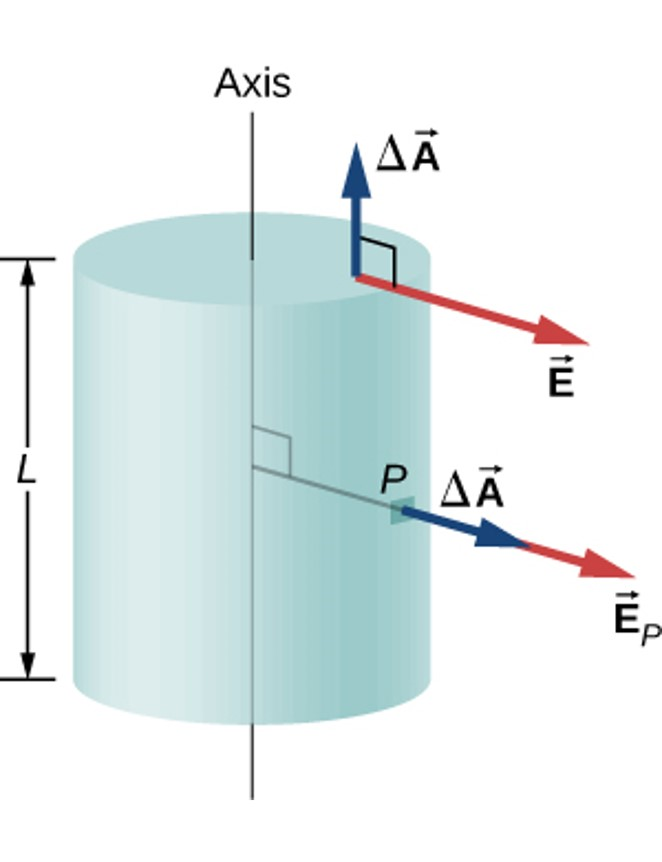
\includegraphics[scale=0.40]{fig/fig_06_29.jpg}
\caption{Cylindrically symmetric of length L}
\label{fig:06_29}
\end{center}
\end{figure}

The electric field is perpendicular to the sides and parallel to the end caps.

The flux through the cylinder part is

\begin{equation}
\int_s \vec{E} \cdot \hat{n} dA = E \int_s dA = E(2 \pi r L)
\end{equation}

and the flux through the caps is zero, because

\begin{equation}
\vec{E} \cdot \hat{n} = 0
\end{equation}

The total flux is then 

\begin{equation}
\int_s \vec{E} \cdot \hat{n} dA = 2 \pi r L E + 0 + 0 = 2 \pi r L E
\end{equation}

Using Gauss's law and taking $\lambda_{enc}$ to be the charge per unit length

\begin{equation}
q_{enc} = \lambda_{enc} L
\end{equation}

\begin{equation}
\Phi = 2 \pi r L E = \frac{q_{enc}}{\epsilon_0}
\end{equation}

The magnitude of $\vec{E}$
\begin{equation}
E(r)  = \frac{\lambda_{enc}}{2 \pi \epsilon_0} \frac{1}{r}
\end{equation}

\begin{equation}
  \lambda_{enc} L =\begin{cases}
    q_{tot}, & \text{if } r \geq R.\\
    q_{(r<R)}, & \text{if } r < R.
  \end{cases}
\end{equation}

What happens of it is a cylindrical shell vs a solid cylinder?

Consider surface charge density of $\sigma$.

\begin{figure}[H]
\begin{center}
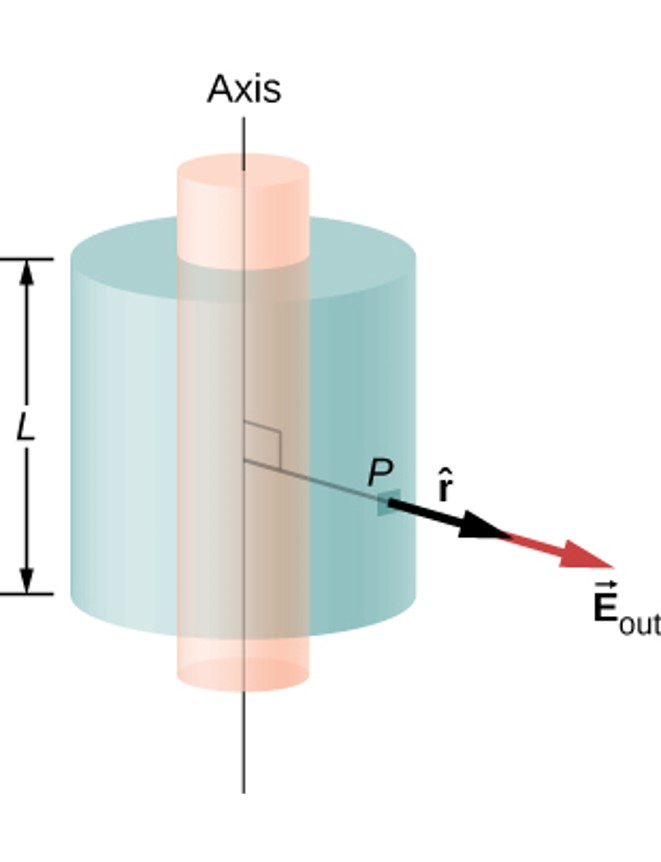
\includegraphics[scale=0.40]{fig/fig_06_30.jpg}
\caption{Guassian surface around a cylinderical shell}
\label{fig:06_30}
\end{center}
\end{figure}

\begin{equation}
\lambda_{enc} = \frac{\sigma 2 \pi R L}{L} = 2 \pi R \sigma
\end{equation} 

For point $P$ outside of the shell $r \geq R$:

\begin{equation}
\vec{E} = \frac{2 \pi R \sigma}{2 \pi \epsilon_0} \frac{1}{r} \hat{r} = \frac{ R \sigma}{ \epsilon_0} \frac{1}{r} \hat{r}
\end{equation}

For point $P$ inside of the shell $r < R$:

\begin{equation}
\lambda_{enc} = 0
\end{equation}

so

\begin{equation}
\vec{E} = 0
\end{equation}

\subsubsection{Planar Symmetry}

\begin{figure}[H]
\begin{center}
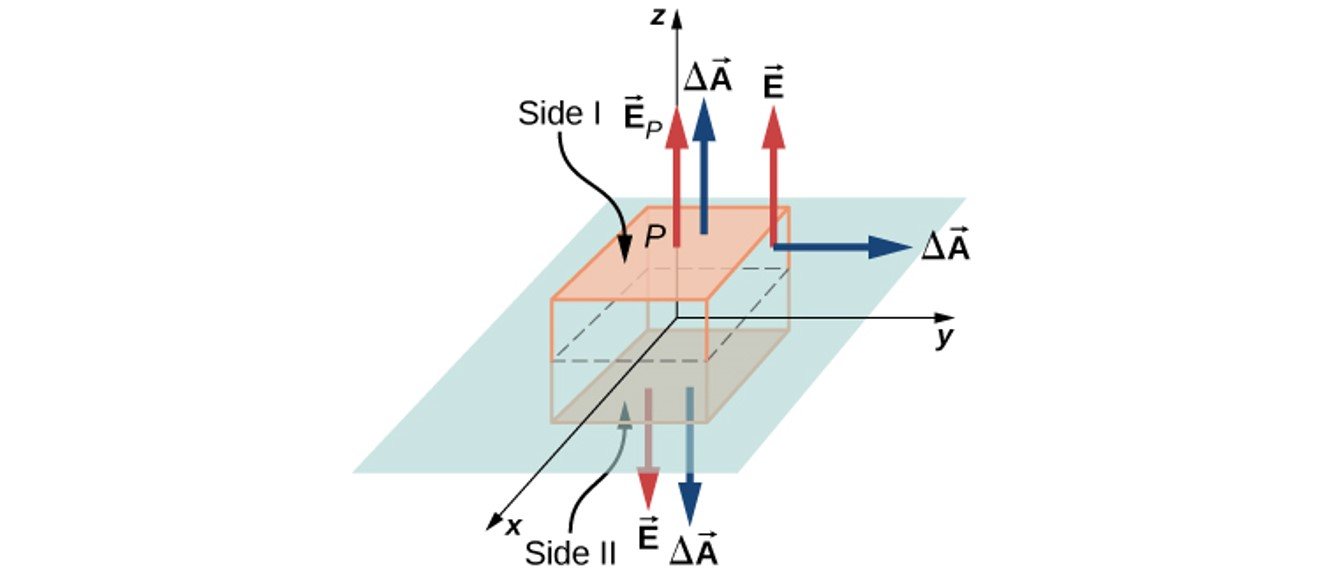
\includegraphics[scale=0.40]{fig/fig_06_33.jpg}
\caption{Thin Charged Sheet}
\label{fig:06_33}
\end{center}
\end{figure}

Consider a large flat surface with uniform charge density. The charge density is the same at all points (x,y), so the electric field $\vec{E}$ at point P only depends on the z-coordinate. 

\begin{equation}
\vec{E} = E(z) \hat{z}
\end{equation}

Note that $E(z) = E(-z)$ thought the direction is opposite. 

Let the electric field at point $P$ be $E_P = E(z)$. If the charge is positive, the field lines point away from the sheet, so

\begin{equation}
\Phi = \oint_S \vec{E}_P \cdot \hat{n} dA = E_P A + E_P A + 0 + 0 +0 + 0 = 2 E_P A
\end{equation}

The charge inside the gaussian box on the plane is 

\begin{equation}
q_{enc} = \sigma A
\end{equation}

Given Gauss's law ($\Phi = \frac{q_{enc}}{\epsilon_0}$) :
\begin{equation}
\frac{q_{enc}}{\epsilon_0} = \frac{\sigma A}{\epsilon_0}
\end{equation}

\begin{equation}
E_P = \frac{\Phi}{2A} = \frac{\sigma}{2 \epsilon_0}
\end{equation}

\begin{equation}
\vec{E}_P = \frac{\sigma}{2 \epsilon_0} \hat{n}
\end{equation}

with $\hat{n} = +\hat{z}$ above the plane and $\hat{n} = -\hat{z}$ below the plane, and $E_P$ doesn't depend on the distance above the plane for an infinite plane. Practically, this is  a useful approximation for a finite plate near the center. 

\section{Conductors in Electrostatic Equilibrium}
Moving from insulators to conductors. The electric field in conductors exerts a force on the free electrons (conduction electrons). As these electrons are not bound to an atom, they accelerate. However, moving charges are not static, so when electrostatic equilibrium is reached the charges are distributed in such a way that the electric field inside the conductor vanishes. 

\subsection{Electric Field inside a Conductor vanishes}

\begin{figure}[H]
\begin{center}
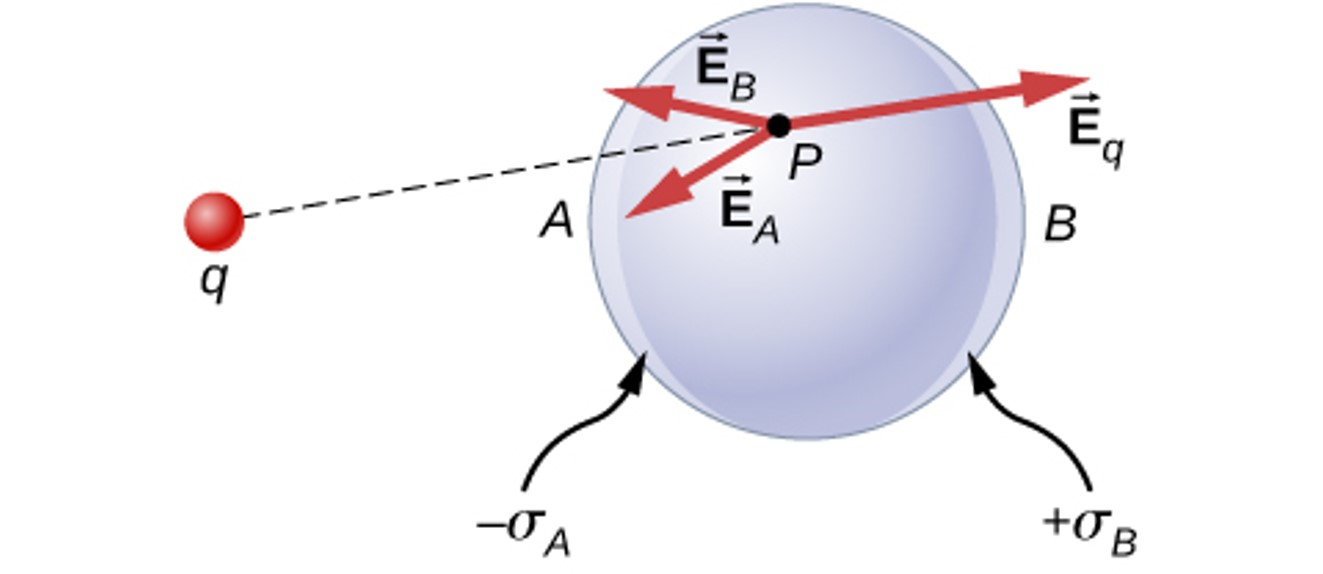
\includegraphics[scale=0.40]{fig/fig_06_35.jpg}
\caption{Metallic Sphere in presence of point charge}
\label{fig:06_35}
\end{center}
\end{figure}


The redistribution of charges is such that 
\begin{equation}
\vec{E}_P = \vec{E}_q + \vec{E}_A + \vec{E}_B = \vec{0}
\end{equation}

for induced charge $-\sigma_A$ and $+\sigma_B$

There is no net charge enclosed by a Gaussian surface that is solely within the volume of a conductor at equilibrium. This gives us $q_{enc} = 0$ and 

The redistribution of charges is such that 
\begin{equation}
\vec{E}_{net} = \vec{0} \text{   at points inside a conductor}
\end{equation}

\subsection{Charge on a conductor}

A consequence of a conductor in static equilibrium is that excess charge will end up on the outer surface of the conductor regardless of its origin.

\begin{figure}[H]
\begin{center}
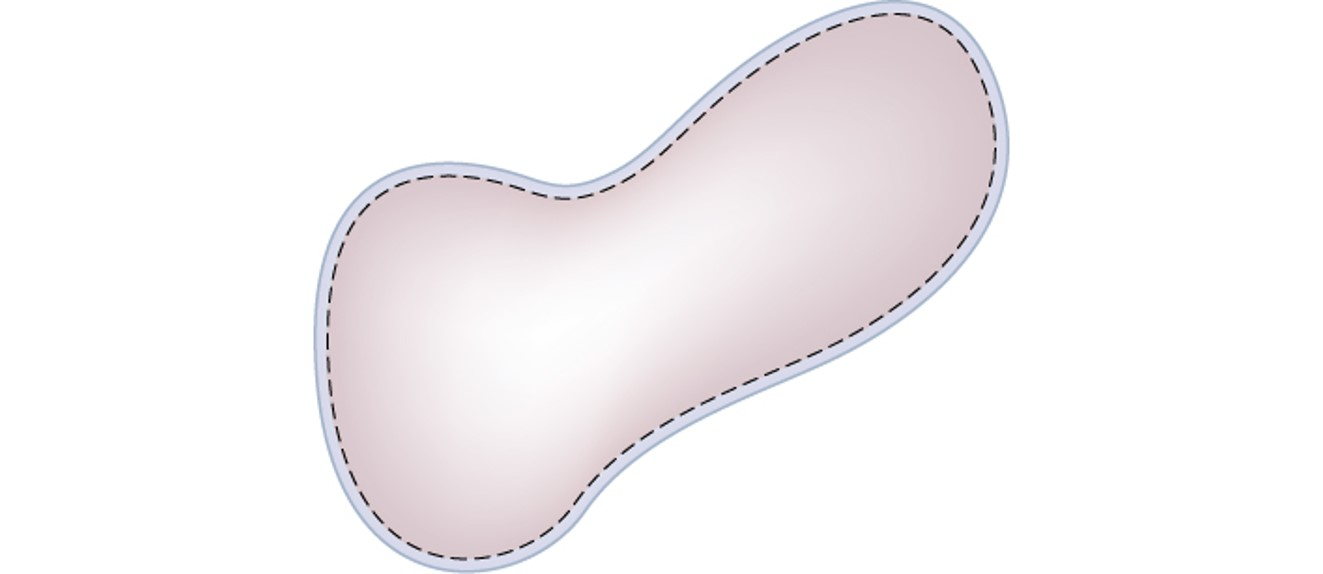
\includegraphics[scale=0.40]{fig/fig_06_37.jpg}
\caption{Gaussian surface just below conductor surface}
\label{fig:06_37}
\end{center}
\end{figure}

Since $E=0$ everywhere inside the conductor, 
\begin{equation}
\oint_s = \vec{E} \cdot \hat{n}dA = 0
\end{equation}

As the Gaussian surface lies infinitesimally below the actual surface, and there is no charge within the Gaussian surface, then all the excess charge must be on the surface. 

\subsection{Electric Field at the Surface of a Conductor}

If the electric field had a component parallel to the surface of the conductor, then the charges would move, which violates the electrostatic equilibrium assuming. Therefor the field must be normal to the surface. 

Just above the surface the magnitude of the electric field ($E$) and the surface charge density ($\sigma$) are related by

\begin{equation}
E = \frac{\sigma}{\epsilon_0}
\end{equation}

\begin{figure}[H]
\begin{center}
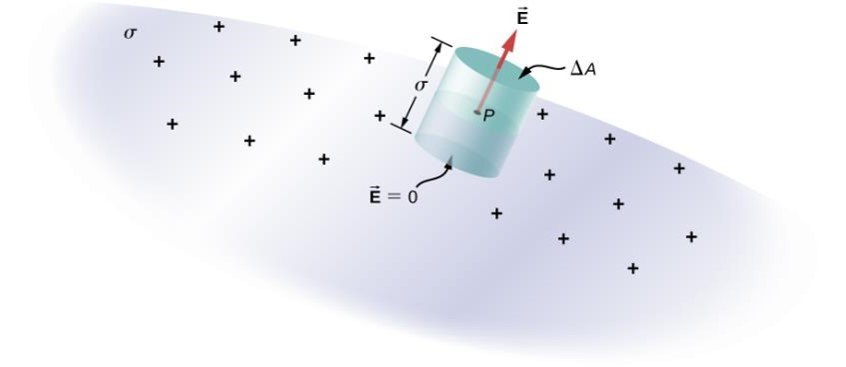
\includegraphics[scale=0.40]{fig/fig_06_39.jpg}
\caption{Field over the surface of a conductor}
\label{fig:06_39}
\end{center}
\end{figure}

Consider an infinitesimally small cylinder on the surface of a conductor with one face inside the conductor and one face outside. The height is $\delta$ and the cross section $\Delta A$. 

Given that $\Delta A$ is infinitesimally small, the total charge in the cylinder is $\sigma \Delta A$. 

The field is perpendicular to the surface, and thus the flux 
\begin{equation}
\Phi = E \Delta A = \frac{\sigma \Delta A}{\epsilon_0}
\end{equation}

yielding that charge right above the surface being given by:

\begin{equation}
E = \frac{\sigma}{\epsilon_0}
\end{equation}

\subsubsection{Electric Field of a Conducting Plate}

\begin{figure}[H]
\begin{center}
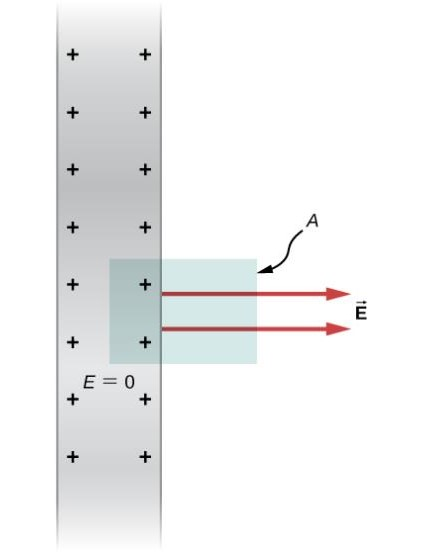
\includegraphics[scale=0.30]{fig/fig_06_40.jpg}
\caption{Conducting Plate}
\label{fig:06_40}
\end{center}
\end{figure}

A conducting plate is similar to the thin conducting plate, however, with $E = 0$ inside the conductor, 

\begin{equation}
\Phi = \oint_S \vec{E}_P \cdot \hat{n} dA = E_P A + 0 + 0 + 0 +0 + 0 =  E_P A
\end{equation}

and thus

\begin{equation}
E = \frac{\sigma}{\epsilon_0}
\end{equation}

\subsubsection{Example: Parallel Plates}

Now consider the electric field between two oppositely charged parallel plates.

If the surface charge density is $\sigma = 6.81 * 10^{-7} \frac{C}{m^2}$ and the distance between the plates is $l = 6.50mm$, what is the electric field? 


\begin{figure}[H]
\begin{center}
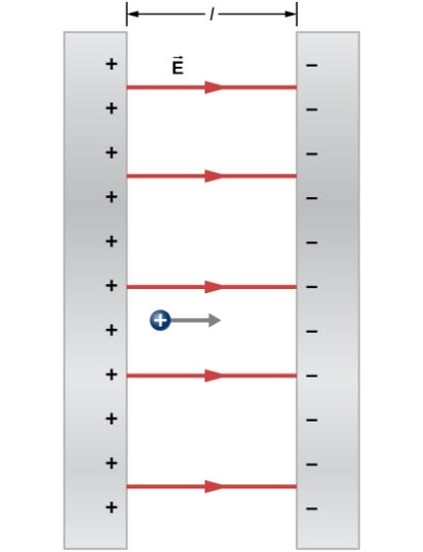
\includegraphics[scale=0.30]{fig/fig_06_41.jpg}
\caption{Between Conducting Plates}
\label{fig:06_41}
\end{center}
\end{figure}

\begin{equation}
E = \frac{\sigma}{\epsilon_0} = \frac{ 6.81 * 10^{-7} \frac{C}{m^2}}{8.85 * 10^{-12}} \frac{C^2}{N \cdot m^2} = 7.69 * 10^{4} \frac{N}{C}
\end{equation}

\chapter{Module 3: Chapter 7 - Electric Potential}

\section{Electric Potential Energy}

\begin{figure}[H]
\begin{center}
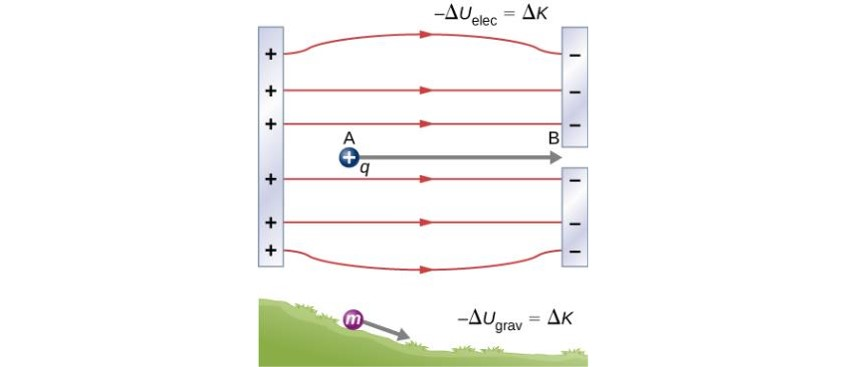
\includegraphics[scale=0.50]{fig/fig_07_02.jpg}
\caption{Charge and Mass in Gravity analogy}
\label{fig:07_02}
\end{center}
\end{figure}

A charge accelerated by an electric field is analogous to a mass going down a hill. Thus, when a free charge is accelerated by an electric field it is also given kinetic energy. This kinetic energy exactly equals the decrease in potential energy

The electrostatic (or Coulomb) force is conservative. This means the work done on charge q is independent of the path taken. 

\begin{figure}[H]
\begin{center}
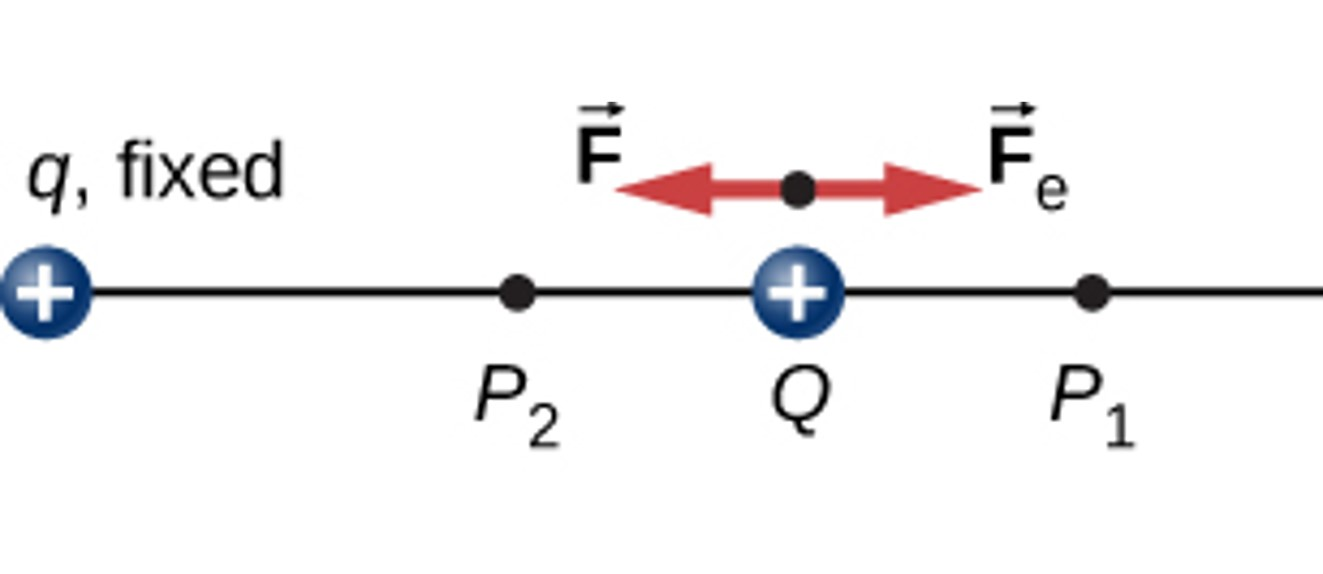
\includegraphics[scale=0.40]{fig/fig_07_03.jpg}
\caption{Displacement of "test" charge Q}
\label{fig:07_03}
\end{center}
\end{figure}

Consider fixed charge $+q$ located at the origin. Push test charge $+Q$ towards $+q$ in such as way that the applied force $\vec{F}$ exactly balances out the electric force $\vec{F}_e$.

In mechanics, $W = mass * displacement$; similarly, for the electric field, the work done moving charge $+Q$ from P1 to P2 is found by

\begin{equation}
W_{12} = \int_{P1}^{P2} \vec{F} \cdot d\vec{I}
\end{equation}

Because $\vec{F}$ balances out $\vec{F}_e$:

\begin{equation}
\vec{F} = -\vec{F}_e = -k\frac{qQ}{r^2}\hat{r} 
\end{equation}

Recalling Coulomb's constant: $k = \frac{1}{4 \pi \epsilon_0} = 8.99 * 10^9 \frac{N \cdot m^2}{C^2}$

Finally, let U denote Potential Energy in Joules ($J = N \cdot m$). Negative work mean gain in potential energy

\begin{equation}
\Delta U = - W
\end{equation}

Because the electrostatic force is conservative, the work $W$ is independent of the path taken. Consider

\begin{figure}[H]
\begin{center}
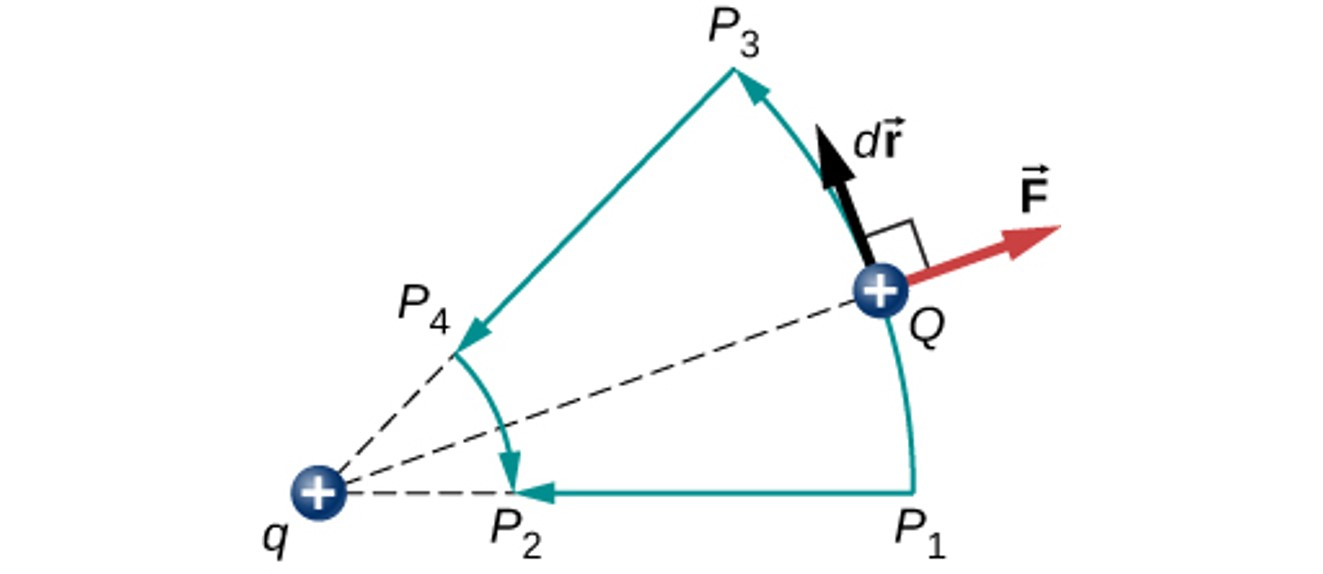
\includegraphics[scale=0.40]{fig/fig_07_05.jpg}
\caption{Work independent of path taken}
\label{fig:07_05}
\end{center}
\end{figure}

The work on path $P_1 P_2$ is equal to the work along path $P_1 P_3 P_4 P_2$. And, in fact, the work on paths $P_1 P_3$ and $P_4 P_2$ are both zero as the $d\vec{r}$ is perpendicular to the electric field along these segments.

\subsubsection{Example}

How much work is required to assemble this charge configuration:

\begin{figure}[H]
\begin{center}
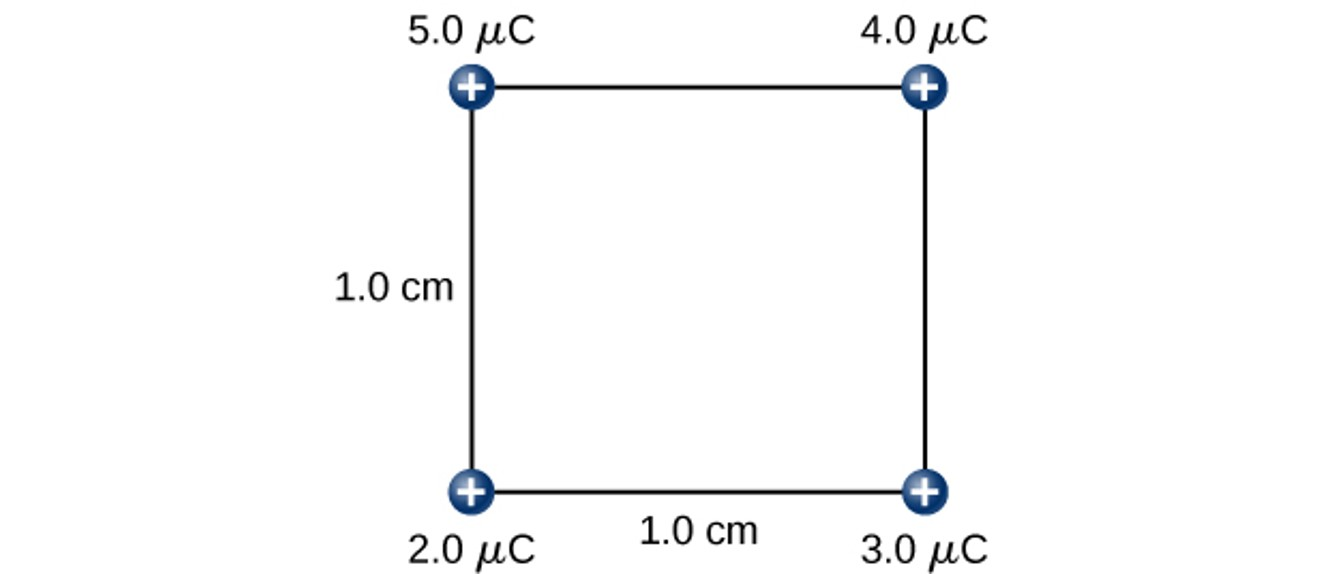
\includegraphics[scale=0.40]{fig/fig_07_08.jpg}
\caption{Work independent of path taken}
\label{fig:07_08}
\end{center}
\end{figure}

\begin{enumerate}


\item Lower left: first bring this $2 \mu C$ charge to the origin. This requires no work as there are no yet any other charges, and thus no electric field. 

\item Lower right: bring $3 \mu C$ charge to (x,y,z) coordinates (1 cm, 0, 0)

\begin{equation}
W_2 = k \frac{q_1 q_2}{r_12} = (9.0 * 10^{9} \frac{N \cdot m^2}{C^2}) \frac{(2* 10^{-6} C) (3* 10^{-6} C) }{1.0 * 10^{2} m} = 5.4 J
\end{equation}

\item Upper right: $r_{23} = 1.0 cm$ and $r_{13} = \sqrt{2.0} cm$

\begin{equation}
W_3 = 15.9 J
\end{equation}

\item Upper left: Similarly, $r_{14} = 1.0 cm$, $r_{34} = 1.0 cm$ and $r_{23} = \sqrt{2} cm$

\begin{equation}
W_4 = 36.5 J
\end{equation}
\end{enumerate}

\begin{equation}
W_{total} = W_1 + W_2 + W_3 + W_4 = 0 + 5.4J + 15.9J + 36.5J = 57.8J
\end{equation}

In general

\begin{equation}
W_{123...N} = \frac{1}{2} k \sum_{i}^{N} \sum_{j}^{N} \frac{q_i q_j}{r_{ij}} \text{ for } i \neq j
\end{equation}

The $\frac{1}{2}$ accounts for each pairing being counted twice. 



\section{Electric Potential and Potential Difference}

The electric field is independent of the test charge. Calculating $W$ directly can be difficult as direction and magnitude of $\vec{F}$ since $W= \vec{F} \cdot \vec{d}$ can be complex for multiple charges, odd shapes, and arbitrary paths. However, because we know $\vec{F} = q \vec{E}$ that the work and hence $\Delta U$ is proportional to the test charge $q$. 

To have a physical quantity independent of the test charge, we define electric potential ($V$):

\begin{equation}
V = \frac{U}{q}
\end{equation}

Since $U \propto q$, then $V$ is independent of $q$. And, we have

\begin{equation}
\Delta V = V_A - V_B = \frac{\Delta U}{q}
\end{equation}

or 

\begin{equation}
\Delta U = q \Delta V
\end{equation}

The units for potential difference $\Delta V$ are Joules per Coulomb, which is referred to as a Volt\footnote{The volt was named after Alessandro Volta}. Whenever voltage is noted, it is understood to be the potential difference between two points. 

Another fundamental constant is that over the electron volt (eV) which is the energy given to the fundamental charge accelerated through a potential difference of 1 volt.

\begin{equation}
1 eV = (1.60 * 10^{-19} C)(1V) = (1.60 * 10^{-19} C)(1 \frac{J}{C}) = 1.60 * 10^{-19} J
\end{equation} 

Due to conservation of energy

\begin{equation}
K + U = \text{constant}
\end{equation}

where $K$ is the Kinetic Energy and $U$ is the Potential Energy

or

\begin{equation}
K_i + U_i = K_f + U_f
\end{equation}

\subsubsection{Example}
Calculate the speed of an electron accelerated through 100V

\begin{equation}
K_i = 0, U_i = qV
\end{equation}

\begin{equation}
K_f = \frac{1}{2}mv^2, U_f = 0
\end{equation}

Thus

\begin{equation}
qV = \frac{1}{2}mv^2
\end{equation}

\begin{equation}
v = \sqrt{\frac{2qV}{m}}
\end{equation}

\begin{equation}
v = \sqrt{\frac{2 (-1.6 * 10^{-19}C)(-100 \frac{J/C})}{9.11*10^{-31} kg}}
\end{equation}

\begin{equation}
v = 5.93 * 10^6 \frac{m}{s}
\end{equation}

\subsection{Voltage and the Electric Field}

Returning to the general formula for the potential energy of a point charge $q$ at Point P relative to a reference Point R.

\begin{equation}
U_P = - \int_{R}^{P} \vec{F} \cdot d\vec{I}
\end{equation}

given that $\vec{F} = q \vec{E}$:

\begin{equation}
U_P = -q \int_{R}^{P} \vec{E} \cdot d\vec{I}
\end{equation}

as we defined $V = \frac{U}{q}$:

\begin{equation}
V_P = - \int_{R}^{P} \vec{E} \cdot d\vec{I}
\end{equation}

From conservation of energy, the result is independent of the path chosen, so we can pick the path that is most convenient. 

\subsubsection{Special Case}

Consider the special case with a positive charge at the origin. To calculate the potential at a point r relative to a potential of 0 at infinity. Let $P = r$, $R = \infty$, $d\vec{I} = d\vec{r} = \hat{r}dr$.

Using $\vec{E} = k\frac{q}{r^2}\hat{r}$:

\begin{equation}
V_r = -\int_{\infty}^r k\frac{q}{r^2} \hat{r} \cdot \hat{r} dr
\end{equation}

\begin{equation}
V_r = -\int_{\infty}^r k\frac{q}{r^2} dr
\end{equation}  

\begin{equation}
V_r = k\frac{q}{r} \bigg\rvert_{\infty}^{r} = k(\frac{q}{r} - \frac{q}{\infty})
\end{equation} 

\begin{equation}
V_r = k\frac{q}{r}
\end{equation} 

Let's calculate the potential difference between two points equidistant for the reference point. 

\begin{figure}[H]
\begin{center}
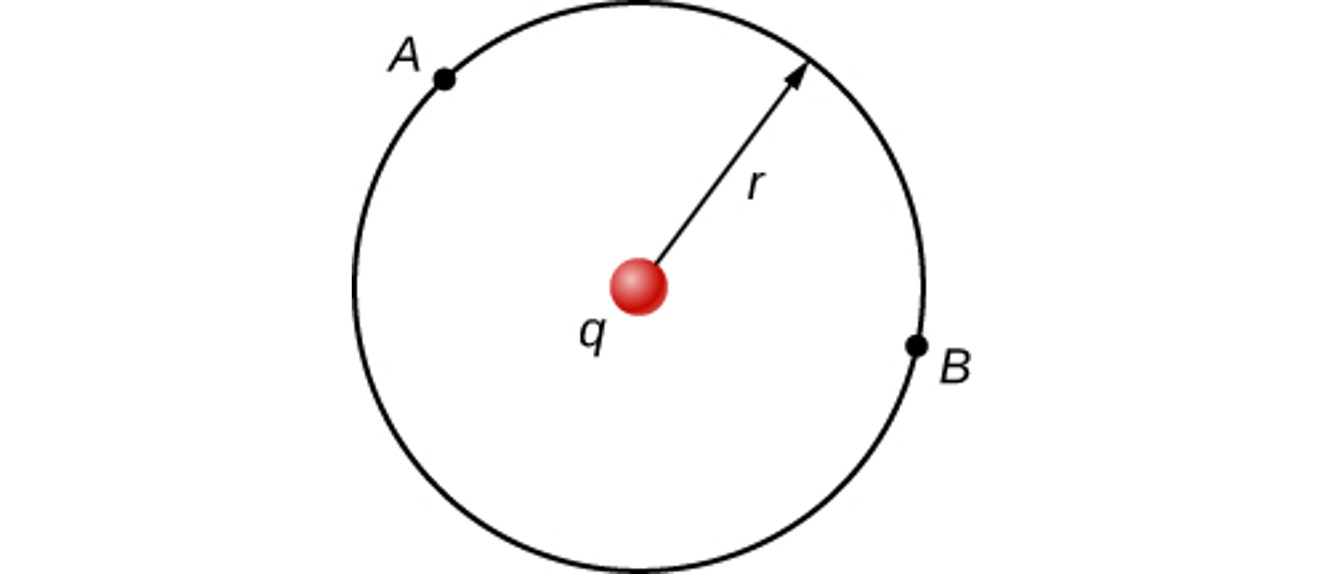
\includegraphics[scale=0.30]{fig/fig_07_15.jpg}
\caption{Potential difference between two equidistant points}
\label{fig:07_15}
\end{center}
\end{figure}

\begin{equation}
\Delta V_{AB} = V_B - V_A = -\int_A^B \vec{E} \cdot d\vec{I}
\end{equation}

\begin{equation}
\Delta V_{AB} =  -\int_A^B \frac{kq}{r^2} \hat{r} \cdot r \hat{\phi} d\phi
\end{equation}

as $\hat{r} \cdot \hat{\phi} = 0$:
\begin{equation}
\Delta V_{AB} =  0
\end{equation}


\begin{figure}[H]
\begin{center}
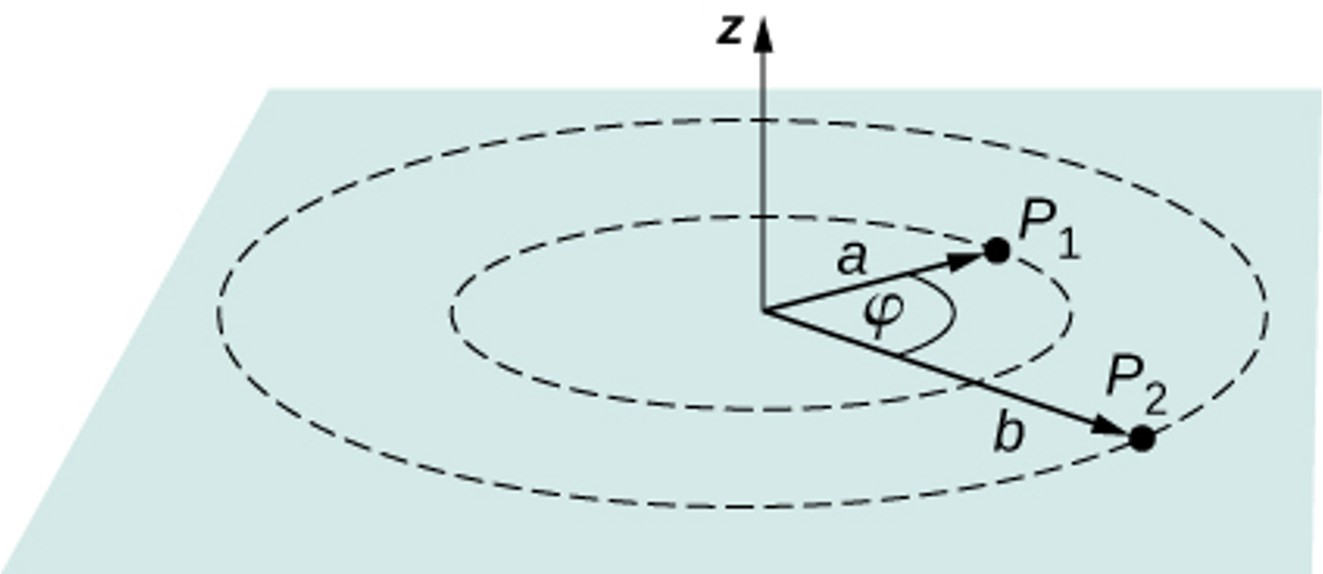
\includegraphics[scale=0.40]{fig/fig_07_17.jpg}
\caption{Potential difference between two points}
\label{fig:07_17}
\end{center}
\end{figure}


\section{Calculations of Electric Potential}

\begin{itemize}
\item From a Point Charge

\begin{equation}
V = \frac{kq}{r}
\end{equation}

\item From multiple Point Charges

\begin{equation}
V = k \sum_{i=1}^{N}\frac{q_i}{i}
\end{equation}

\item From a continuous charge

\begin{equation}
V = k \int \frac{dq}{r}
\end{equation}

\end{itemize}

where

\begin{equation}
  dq = \begin{cases}
    \lambda dl \text{      (in one dimension)} \\
    \sigma dA \text{    (in two dimensions)} \\
    \rho dV \text{    (in three dimensions)} 
  \end{cases}
\end{equation}

\subsubsection{Potential due to a ring}

Consider a disk with uniform charge density $\lambda$ (Coulombs per meter arc length). Let's find the electric potential at a point on the axis passing through the center of the ring. 

\begin{figure}[H]
\begin{center}
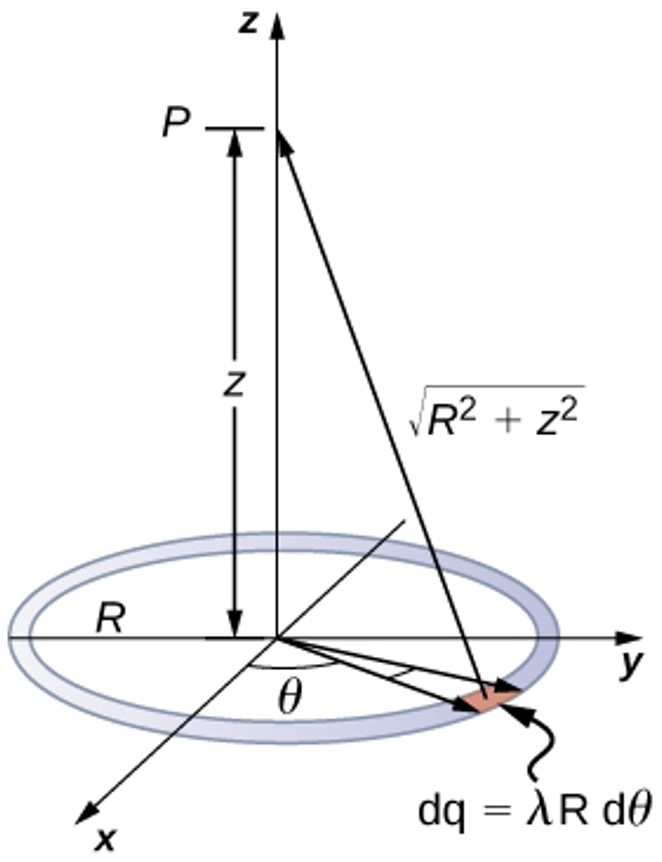
\includegraphics[scale=0.40]{fig/fig_07_24.jpg}
\caption{Ring of charge}
\label{fig:07_24}
\end{center}
\end{figure}

The strategy is to divide the ring into infinitesimal elements shaped as arcs on the circle and to utility cylindrical coordinate system.

The element between angles  $\theta$ and $\theta + d\theta$ is of length $R d\theta$. It therefore contains charge $\lambda R d\theta$. The element is at distance $\sqrt{z^2 + R^2}$ from point P. Therefore:

\begin{equation}
V_P = k \int \frac{dq}{r} = k \int_0^{2\pi} \frac{\lambda R d\theta}{\sqrt{z^2 + R^2}} = \frac{k \lambda R}{\sqrt{z^2 + R^2}} \int_0^{2\pi} d\theta
\end{equation}

\begin{equation}
 = \frac{k \lambda R}{\sqrt{z^2 + R^2}} \theta \bigg\rvert_{0}^{2\pi} = \frac{2 \pi k \lambda R}{\sqrt{z^2 + R^2}} = k \frac{q_{tot}}{\sqrt{z^2 + R^2}}
\end{equation}

\subsubsection{Potential due to a disk}

Consider a disk with uniform charge density $\sigma$ (Coulombs per meter squared). Let's find the electric potential at a point on the axis passing through the center of the disk. 

\begin{figure}[H]
\begin{center}
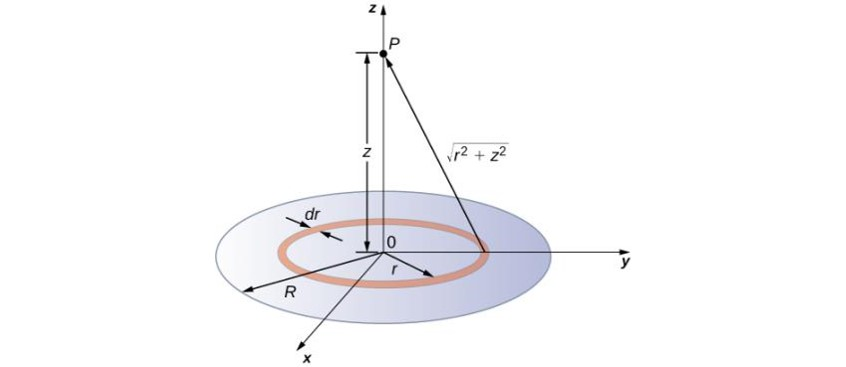
\includegraphics[scale=0.50]{fig/fig_07_25.jpg}
\caption{Disk of charge}
\label{fig:07_25}
\end{center}
\end{figure}

The strategy is to divide the disk into ring-shaped elements, then taking the previous result integrate over $r$ as well as $\theta$.

The infinitesimal width ring elements between cylinder $r$ and $r + dr$ will be a ring of charges whole electric potential $dV_P$ at the field point that is

\begin{equation}
dV_P = k \frac{dq}{\sqrt{z^2 + R^2}}
\end{equation}

where
\begin{equation}
dq = \sigma 2\pi r dr
\end{equation}

Integrating from r = 0 to r = R
\begin{equation}
V_P = \int dV_P = k2\pi\sigma \int_0^R \frac{rdr}{\sqrt{z^2 + r^2}} 
\end{equation}

\begin{equation}
= k2\pi\sigma {\sqrt{z^2 + r^2}} \bigg\rvert_{0}^{R} = k2\pi\sigma (\sqrt{z^2 + R^2}-\sqrt{z^2})
\end{equation}

\section{Determining Field From Potential}

Recall that

\begin{equation}
U = V_B - V_A = \int_A^B \vec{E} \cdot ds
\end{equation}

The electric field can be calculated by taking the derivative of U

For a uniform electric field

\begin{equation}
E = -\frac{\Delta V}{\Delta s}
\end{equation}

where $\Delta s$ is the distance over which the change in potential $\Delta V$ takes place.

For a continuously changing field, $\Delta V$ and $\Delta s$ become infinitesimally small giving 

\begin{equation}
E_s = -\frac{dV}{ds}
\end{equation}


\begin{figure}[H]
\begin{center}
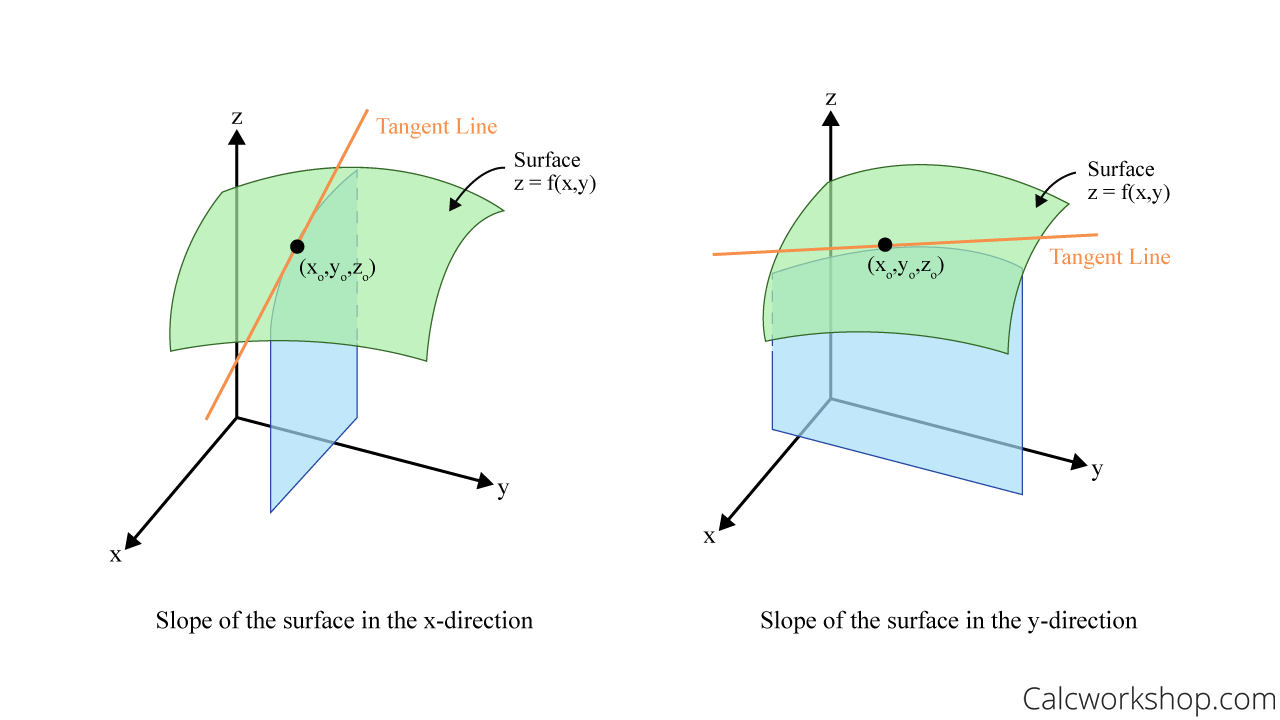
\includegraphics[scale=0.30]{fig/partialderivative.png}
\caption{Partial Derivatives}
\label{fig:pder}
\end{center}
\end{figure}

Using Partial Derivatives, the electric field components in the Cartesian directions are given by

\begin{equation}
E_x = -\frac{\delta V}{\delta x}, E_y = -\frac{\delta V}{\delta y}, E_z = -\frac{\delta V}{\delta z}
\end{equation}

Introducing the Gradient (grad) or Delta (del) vector operator:

\begin{equation}
\vec{\nabla} = \hat{i} \frac{\delta}{\delta x} + \hat{j} \frac{\delta}{\delta y} + \hat{k} \frac{\delta}{\delta k}
\end{equation}

and thus

\begin{equation}
\vec{E} = -\vec{\nabla}V
\end{equation}

For symmetric systems
\begin{itemize}
\item Cylindrical:
\begin{equation}
\vec{\nabla} = \hat{r} \frac{\delta}{\delta r} + \hat{\phi} \frac{1}{r}\frac{\delta}{\delta \phi} + \hat{z} \frac{\delta}{\delta z}
\end{equation}
\item Spherical:
\begin{equation}
\vec{\nabla} = \hat{r} \frac{\delta}{\delta r} + \hat{\theta} \frac{1}{r}\frac{\delta}{\delta \theta} + \hat{\phi} \frac{1}{r\sin{\theta}}\frac{\delta}{\delta \phi}
\end{equation}
\end{itemize}

\subsubsection{Example}

Electric Field of a point charge

\begin{equation}
V = k\frac{q}{r} \text{(spherically symetric)}
\end{equation}

\begin{equation}
\vec{E} = -\vec{\nabla}V
\end{equation}

\begin{equation}
\vec{E} = - (\hat{r} \frac{\delta}{\delta r} + \hat{\theta} \frac{1}{r}\frac{\delta}{\delta \theta} + \hat{\phi} \frac{1}{r\sin{\theta}}\frac{\delta}{\delta \phi}) k\frac{q}{r}
\end{equation}

\begin{equation}
\vec{E} = - kq (\hat{r} \frac{\delta}{\delta r} (\frac{1}{r}) + \hat{\theta} \frac{1}{r}\frac{\delta}{\delta \theta} (\frac{1}{r}) + \hat{\phi} \frac{1}{r\sin{\theta}}\frac{\delta}{\delta \phi}(\frac{1}{r}))
\end{equation}

\begin{equation}
\vec{E} = - kq (\hat{r}  (\frac{-1}{r^2}) + \hat{\theta} (0) + \hat{\phi} (0))
\end{equation}

\begin{equation}
\vec{E} = + \frac{kq}{r^2} \hat{r}  
\end{equation}

\begin{figure}[H]
\begin{center}
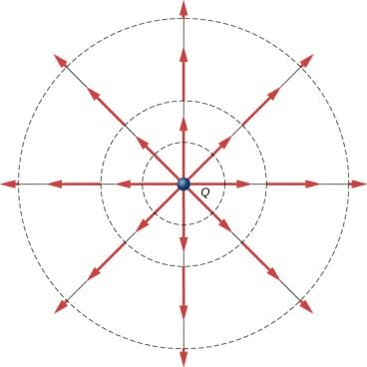
\includegraphics[scale=0.40]{fig/fig_07_28.jpg}
\caption{Electric Field from Point Charge}
\label{fig:07_28}
\end{center}
\end{figure}

\subsubsection{Electric Field from Ring of Charge}

\begin{figure}[H]
\begin{center}
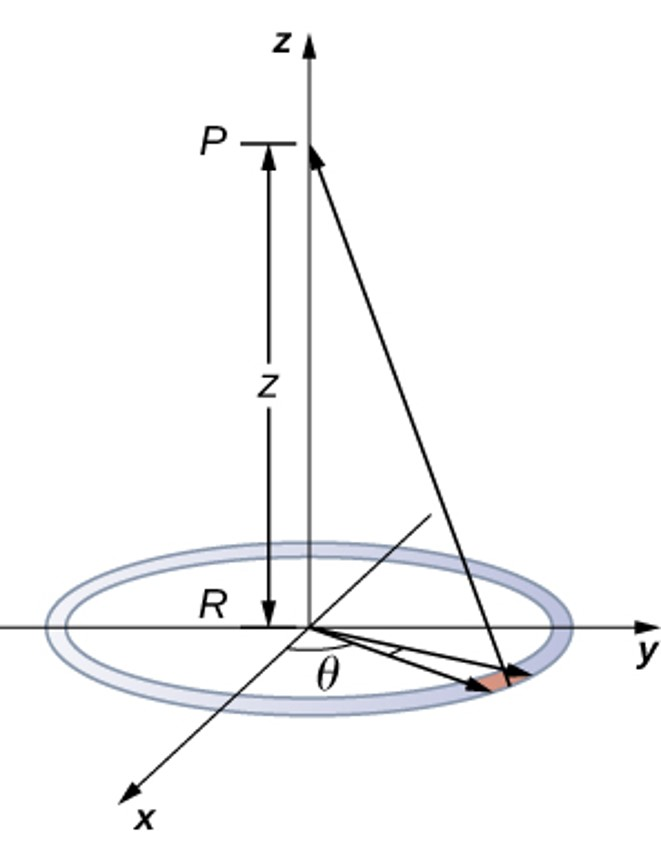
\includegraphics[scale=0.40]{fig/fig_07_29.jpg}
\caption{Electric Field from Ring Of Charge}
\label{fig:07_29}
\end{center}
\end{figure}

\begin{equation}
E_z = -\frac{\delta V}{\delta z} \text{ with } V = k\frac{k q_{tot}}{\sqrt{z^2+R^2}}
\end{equation}

\begin{equation}
E_z = -\frac{\delta}{\delta z} (k\frac{k q_{tot}}{\sqrt{z^2+R^2}})
\end{equation}

Given that
\begin{equation}
\frac{\delta}{\delta z} (\frac{1}{\sqrt{z^2+R^2}}) = \frac{\delta}{\delta z} (z^2+R^2)^{-\frac{1}{2}} = -\frac{1}{2} (z^2+R^2)^{-\frac{3}{2}} (2z)
\end{equation}

We get
\begin{equation}
E_z = +k \frac{k q_{tot} z}{(z^2+R^2)^{\frac{3}{2}}}
\end{equation}

\section{Electropotential Surfaces and Conductors}

\begin{figure}[H]
\begin{center}
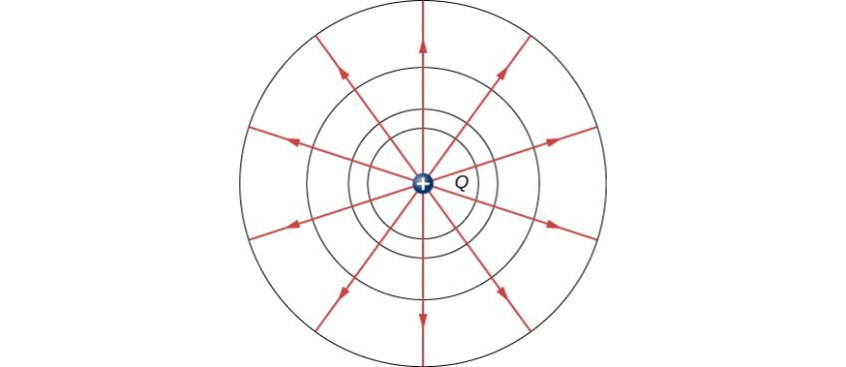
\includegraphics[scale=0.50]{fig/fig_07_30.jpg}
\caption{Red: Field Lines, Blue: Equipotential Lines}
\label{fig:07_30}
\end{center}
\end{figure}

Equipotential Lines are always perpendicular to the electric field lines since along them $\Delta V = 0$.

\begin{equation}
W = -\Delta U = -q \Delta V = 0
\end{equation}

Work is zero when the direction of the force is perpendicular to displacement.

\begin{equation}
W = \vec{F} \cdot \vec{d} = q\vec{E} \cdot \vec{d} = qEd\cos{\theta} \text{ for } \theta = 90^{\circ} \text{ or } 270^{\circ}
\end{equation}


\subsection{Conductors}

\begin{itemize}
\item One of the rules for static electric fields and conductors is that the $\vec{E}$ is perpendicular ($\bot$) to the surface.
\item This implies that a conductor is an equipotential surface in static situations. There
can be no voltage difference across the surface of a conductor, or charges will flow. 
\item One of the uses of this fact is that a conductor can be fixed at what we consider zero volts by connecting it to the earth with a good conductor — a process called grounding.
\end{itemize}

Because a conductor is an equipotential, it can replace any equipotential surface. For example, a charged spherical conductor can replace the point charge, and the electric field and potential surfaces outside of it will be unchanged, confirming the contention that a spherical charge distribution is equivalent to a point charge at its center.

\begin{figure}[H]
\begin{center}
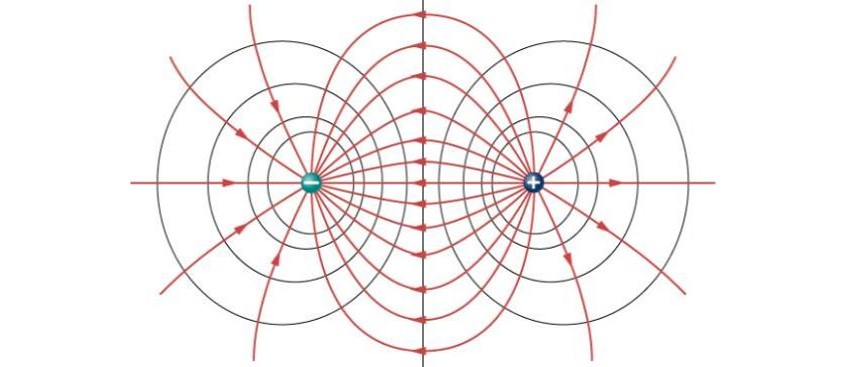
\includegraphics[scale=0.50]{fig/fig_07_31.jpg}
\caption{Potential lines, two opposite charges}
\label{fig:07_31}
\end{center}
\end{figure}



\begin{figure}[H]
\begin{center}
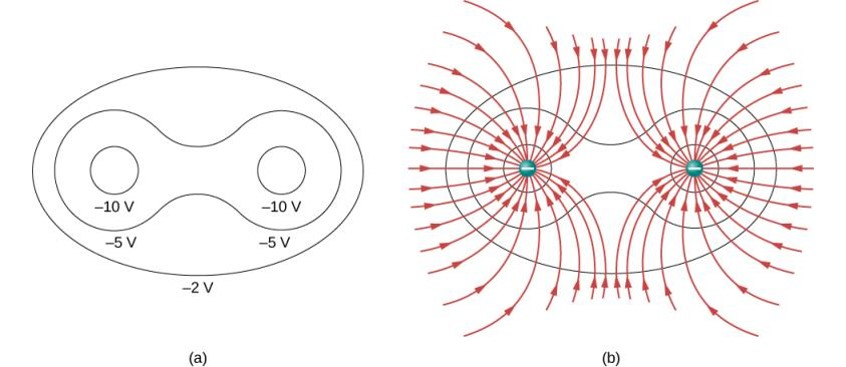
\includegraphics[scale=0.50]{fig/fig_07_32.jpg}
\caption{Equipotential lines (as might be measured by a voltmeter) and corresponding electric field}
\label{fig:07_32}
\end{center}
\end{figure}

One of the most important cases is that of the familiar parallel conducting plates. Between the plates, the equipotentials are evenly spaced and parallel. The same field could be maintained by
placing conducting plates at the equipotential lines at the potentials shown.

\begin{figure}[H]
\begin{center}
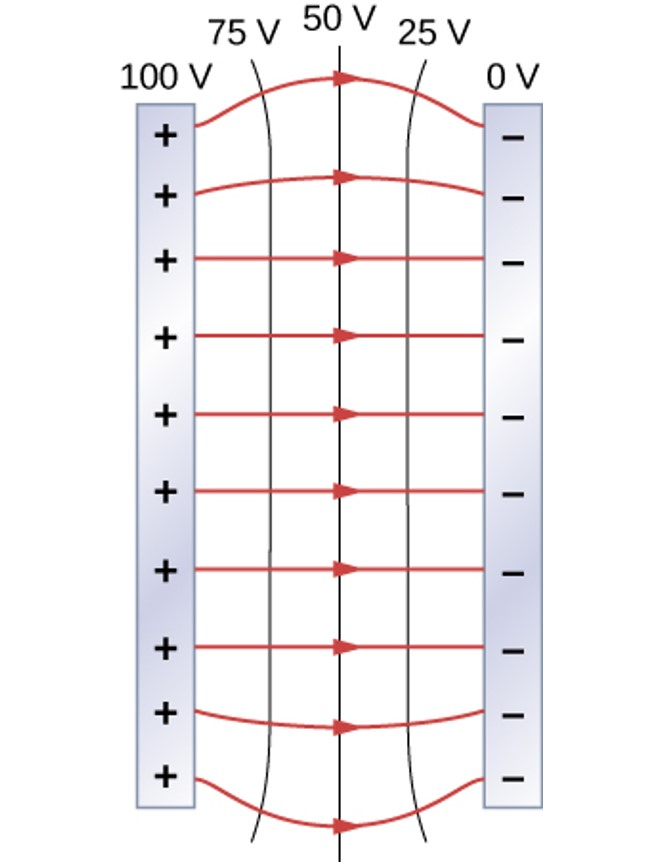
\includegraphics[scale=0.50]{fig/fig_07_35.jpg}
\caption{Two parallel plates - $\vec{E}$ and equipotential lines}
\label{fig:07_35}
\end{center}
\end{figure}

\subsubsection{Examples}

Consider Figure \ref{fig:07_30} with $Q = +10nC$ at the Origin. What are the equipotential surfaces at which the potential is:

\begin{enumerate}[(a)]
\item 100V
\item 50V
\item 20V
\item 10V
\end{enumerate}

For $V = k\frac{q}{r}$, V is a constant. Thus, $r = k\frac{q}{V}$.

\begin{enumerate}[(a)]
\item 100V: $r = k\frac{q}{V} = (8.99 * 10^9 \frac{Nm^2}{C^2}) \frac{10 * 10^{-9} C}{100V} = 0.90m$
\item 50V $r = 1.8m$
\item 20V $r = 4.5m$
\item 10V $r = 9.0m$
\end{enumerate}


\begin{figure}[H]
\begin{center}
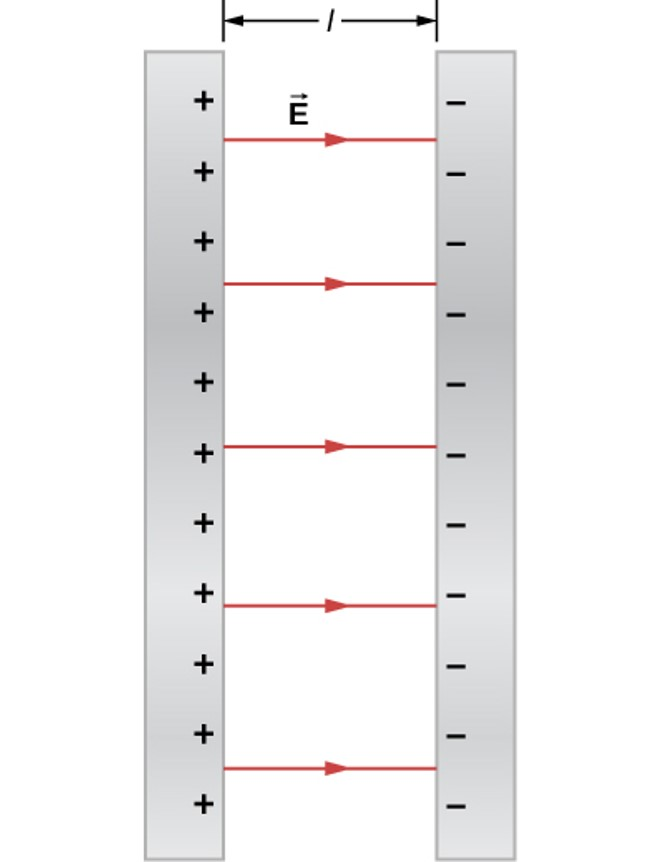
\includegraphics[scale=0.50]{fig/fig_07_37.jpg}
\caption{Oppositely charged parallel plates}
\label{fig:07_37}
\end{center}
\end{figure}

Two large conducting plates carry equal and opposite charges, with a surface charge density $\sigma = 6.81 * 10^{-7} \frac{C}{m^2}$ of magnitude as shown in Figure \ref{fig:07_37}. The separation between the plates is $l = 6.5mm$ 
\begin{enumerate}[(a)]
\item What is the electric field between the plates? 
\item What is the potential difference between the plates? 
\item What is the distance between equipotential planes which differ by 100 V?
\end{enumerate}

Assume the size of the plates ($L$) is much larger than the distance $l$.

\begin{equation}
\Delta V_{AB} = - \int_A^B \vec{E} \cdot d\vec{I}
\end{equation}

\begin{enumerate}[(a)]
\item Electric Field is directed from +plate to the -plate with magnitude
	\begin{equation}
	E = \frac{\sigma}{\epsilon_0} = \frac{6.81 * 10^{-7} \frac{C}{m^2}}{8.85 * 10^{-12} \frac{C^2}		{N m^2}} = 7.69 * 10^{4} \frac{V}{m}
	\end{equation}
\item The path from -plate to +plate is directed against $\vec{E}$
	\begin{equation}
	\vec{E} = d\vec{I} = -E \cdot dl
	\end{equation}
	
	\begin{equation}
	\Delta V = \int E \cdot dl = E \int dl = El = (7.69 * 10^{4} \frac{V}{m})(6.5 * 10^{-3}m) = 		500V
	\end{equation}
	
\item Uniform electric field 
	\begin{equation}
	\frac{500V}{6.5 * 10^{-3}m} = \frac{100V}{x}
	\end{equation}
	
	\begin{equation}
	x = 1.3 * 10^{-3}m
	\end{equation}
\end{enumerate}

\begin{figure}[H]
\begin{center}
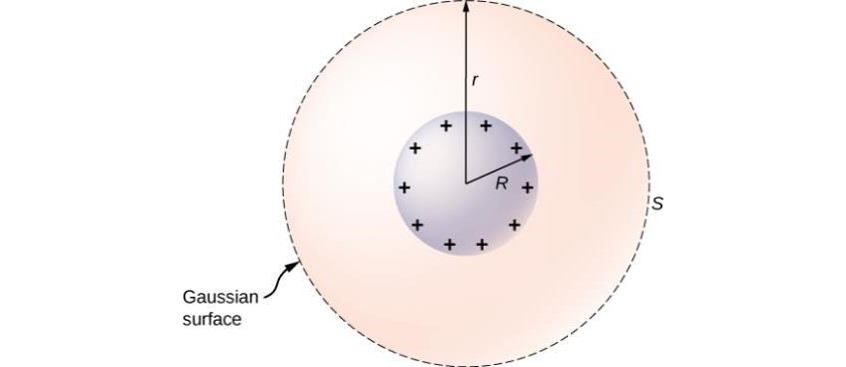
\includegraphics[scale=0.50]{fig/fig_07_38.jpg}
\caption{An isolated conducting sphere}
\label{fig:07_38}
\end{center}
\end{figure}

\begin{equation}
\vec{E} = E(r) \hat{r} 
\end{equation}

Applying Gauss's Law over a closed surface s of radius r. As $r$ = a constant, $\hat{r} = \hat{n}$ on the surface of the sphere. 

\begin{equation}
\oint_s \vec{E} \cdot \hat{n} = E(r) \oint_s da = E(r) 4 \pi r^2
\end{equation} 

For $r < R$: s in inside the conductor.

Magnitude
\begin{equation}
E(r) = \frac{1}{4 \pi \epsilon_0} \frac{q_{enc}}{r^2}
\end{equation}

\begin{equation}
q_{enc} = 0 \Rightarrow E(r) = 0
\end{equation}

For $r \geq R$: s encloses the conductor so $q_{enc} = q$

\begin{equation}
E(r) = \frac{1}{4 \pi \epsilon_0} \frac{q}{r^2}
\end{equation}

Electric Field
\begin{equation}
  \vec{E} =\begin{cases}
    0 & (r < R)\\
    \frac{1}{4 \pi \epsilon_0} \frac{q}{r^2} \hat{r} & (r \geq R)
  \end{cases}
\end{equation}

Potential 
\begin{itemize}
\item For $r < R$ , $E = 0 \Rightarrow V(r)$ is constant, since $V(R) = \frac{1}{4 \pi \epsilon_0} \frac{q}{R}$


\item For $r \geq R$, potential is the same as a point charge: $V(R) = \frac{1}{4 \pi \epsilon_0} \frac{q}{r}$
\end{itemize}


\begin{figure}[H]
\begin{center}
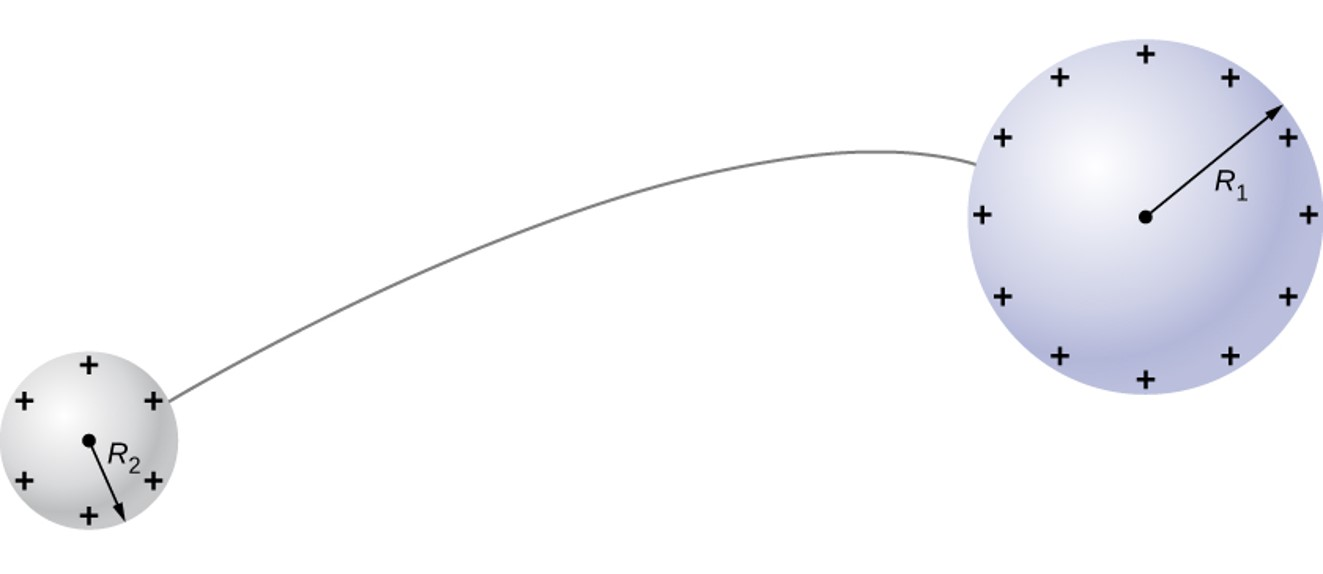
\includegraphics[scale=0.50]{fig/fig_07_39.jpg}
\caption{Two different radii}
\label{fig:07_39}
\end{center}
\end{figure}

Now consider two conducting spheres of radii $R_1$ and $R_2$ connected by a thin conducting wire as shown in Figure \ref{fig:07_39}

\begin{equation}
V = \frac{1}{4 \pi \epsilon_0} \frac{q}{R}
\end{equation}

Given that because of the conducting wire $V_1 = V_2$

\begin{equation}
\frac{1}{4 \pi \epsilon_0} \frac{q_1}{R_1} = \frac{1}{4 \pi \epsilon_0} \frac{q_2}{R_2}
\end{equation}

\begin{equation}
\frac{q_1}{R_1} = \frac{q_2}{R_2}
\end{equation}

Charge surface density $\sigma$: 
\begin{equation}
q = \sigma(4 \pi R^2)
\end{equation}

Substituting in for $q_1$ and $q_2$ and simplifying

\begin{equation}
\sigma_1 R_1 = \sigma_2 R_2
\end{equation}

\subsubsection{Different Radii of Curvature on the same object}

\begin{figure}[H]
\begin{center}
\includegraphics[scale=0.50]{fig/fig_07_40.jpg}
\caption{Radius of Curvature}
\label{fig:07_40}
\end{center}
\end{figure}

Different Radii of Curvature on the same object
\begin{itemize}
\item Large Radius of Curvature $\Rightarrow \sigma \text{ and } E$ are small
\item Point $\Rightarrow \sigma \text{ and } E$ are extremely large
\end{itemize}

\subsubsection{Lightning Rod}

On a very sharply curved surface, such as shown in \ref{fig:07_4x}, the charges are so concentrated at the point that the resulting electric field can be great enough to remove them from the surface. This can be useful.

Lightning rods work best when they are most pointed. The large charges created in storm clouds induce an opposite charge on a building that can result in a lightning bolt hitting the building. The induced charge is bled away continually by a lightning rod, preventing the more dramatic lightning strike.

\begin{figure}[H]
\begin{center}
\includegraphics[scale=0.50]{fig/fig_07_4x.jpg}
\caption{Lightning Rod}
\label{fig:07_4x}
\end{center}
\end{figure}

\chapter{Module 4 - Chapter 8 Capacitance}

\section{Capacitors and Capacitance}

A capacitor is a device used to store electrical charge and electrical energy. Capacitors are generally with two electrical conductors separated by a distance. The space is usually
filled with an insulating material known as a dielectric. The amount of storage in a capacitor is referred to as its capacitance. 

\begin{figure}[H]
\begin{center}
\includegraphics[scale=0.50]{fig/fig_08_03.jpg}
\caption{Parallel Plate Capacitor}
\label{fig:08_03}
\end{center}
\end{figure}



\begin{equation}
C = \frac{Q}{V}
\label{eq:cap}
\end{equation}

Capacitance is measured in the Farad\footnote{Named after Michael Farday} (F). One farad is one coulomb per volt: $1 F = \frac{1 C}{1 V}$. 

\subsection{Calculation of Capacitance}
\begin{enumerate}
\item Assume that the capacitor has charge Q
\item Determine the electric field $\vec{E}$
\item Find the potential between the conductors from
	\begin{equation}
	V_B - V_A = - \int_A^B \vec{E} \cdot d\vec{I}
	\label{eq:potcon}
	\end{equation}
	which leads to magnitude of the potential difference being $V = \left| V_B - V_A \right|$.
\item Find $C$ from Equation \ref{eq:cap}
\end{enumerate}

\subsection{Parallel Plate Capacitor}
Consider a parallel plate capacitor with each plate of area $A$ separated by distance $d$. Assume when voltage $V$ is applied, it stores charge $Q$. 

Define the surface charge density $\sigma$ as
\begin{equation}
\sigma = \frac{Q}{A}
\end{equation}

When $d$ is small compared to the size of the plates, the electric field between the plates is fairly uniform, with a magnitude give by:
\begin{equation}
E = \frac{\sigma}{\epsilon_0}
\end{equation}

Since the electric field $\vec{E}$ between the plates is uniform
\begin{equation}
V = Ed = \frac{\sigma d}{\epsilon_0} = \frac{Q d}{\epsilon_0 A}
\end{equation}

From Equation \ref{eq:cap}:
\begin{equation}
C = \frac{Q}{V} = \frac{Q}{\frac{Q d}{\epsilon_0 A}} = \epsilon_0 \frac{A}{d}
\label{eq:qv}
\end{equation}

\subsection{Cylindrical Capacitor}

\begin{figure}[H]
\begin{center}
\includegraphics[scale=0.50]{fig/fig_08_07.jpg}
\caption{Cylindrical Capacitor}
\label{fig:08_07}
\end{center}
\end{figure}

Consider the cylindrical capacitor with the inner cylinder (either solid or shell) of outer radius $r_1$ and out cylinder of inner radius $r_2$. Assume the length is $l$ and the excess charges $+Q$ and $-Q$ are on the inner and outer cylinders, respectively.

Ignoring the edge effect, the electric field $\vec{E}$ radiates out radially from the common axis of the two cylinders. Using the Gaussian Surface shown in Figure \ref{fig:08_07}, yields
\begin{equation}
\oint_S \vec{E} \cdot \vec{n} dA = E(2 \pi r l) = \frac{Q}{\epsilon_0}
\end{equation} 

Therefore, the field between the two cylinders is
\begin{equation}
\vec{E} = \frac{1}{2 \pi \epsilon_0} \frac{Q}{r l} \hat{r}
\end{equation}

Substituting into Equation \ref{eq:potcon}:
\begin{equation}
V = \int_{R_1}^{R_2} \vec{E} \cdot d\vec{I} = \frac{Q}{2 \pi \epsilon_0 l} \int_{R_1}^{R_2} \frac{1}{r} \hat{r} \cdot (\hat{r} dr) = \frac{Q}{2 \pi \epsilon_0 l} \int_{R_1}^{R_2} \frac{dr}{r} 
\end{equation}

\begin{equation}
= \frac{Q}{2 \pi \epsilon_0 l} \ln{(r)}\bigg\rvert_{R_1}^{R_2} =  \frac{Q}{2 \pi \epsilon_0 l}  \ln{(\frac{R_2}{R_1})}
\end{equation}

Thus
\begin{equation}
C = \frac{Q}{V} = \frac{2 \pi \epsilon_0 l}{\ln{(\frac{R_2}{R_1})}}
\end{equation}

This is sometimes expressed at capacitance per unit length 
\begin{equation}
\frac{C}{l} = \frac{2 \pi \epsilon_0 }{\ln{(\frac{R_2}{R_1})}}
\end{equation}

\section{Capacitors in Series and Parallel}  

\subsection{Capacitors in Series}

When a series of capacitors are hooked up to a direct current voltage source (e.g., a battery) each acquires an identical charge $Q$. 

\begin{itemize}
\item The plate connected to the positive terminal acquires a charge $Q$. And, the plate connected to the negative terminal acquires a charge $-Q$. 
\item A charge is then induced on each of the other plates so that the sum of the charge on all plates or on any pair of plates is zero.
\item However, the potential drop on one pair of plates ($V_1=\frac{Q}{C_1}$) may be different from a the drop across another pair of plates ($V_2=\frac{Q}{C_2}$)
\end{itemize}

\begin{figure}[H]
\begin{center}
\includegraphics[scale=0.45]{fig/fig_08_11.jpg}
\caption{Capacitors in Series}
\label{fig:08_11}
\end{center}
\end{figure}

The potentials must sum to the potential of the battery:
\begin{equation}
V = V_1 + V_2 + V_3
\end{equation}

The potential $V$ is measured across a equivalent capacity holding charge $Q$, which is said to have an equivalent capacitance $C_{EQ}$. Leading to:
\begin{equation}
\frac{Q}{C_{EQ}} = \frac{Q}{C_{1}} + \frac{Q}{C_{2}} + \frac{Q}{C_{3}}
\end{equation}

Thus:
\begin{equation}
\frac{1}{C_{EQ}} = \frac{1}{C_{1}} + \frac{1}{C_{2}} + \frac{1}{C_{3}}
\end{equation}



\subsection{Capacitors in Parallel}

If, instead, the three capacitors are connected in parallel, they will have the same voltage across each pair of plates
\begin{equation}
V = V_1 + V_2 + V_3
\end{equation}

\begin{figure}[H]
\begin{center}
\includegraphics[scale=0.60]{fig/fig_08_12.jpg}
\caption{Capacitors in Parallel}
\label{fig:08_12}
\end{center}
\end{figure}

The total charge stored across the plates $Q$ is the equivalent of the sum of the charges on each plate

\begin{equation}
Q = Q_1 + Q_2 + Q_3
\end{equation}

Given that $Q = C * V$:

\begin{equation}
C_{EQ}V = C_{1}V + C_{2}V + C_{3}V
\end{equation}

And, thus:

\begin{equation}
C_{EQ} = C_{1} + C_{2} + C_{3}
\end{equation}


\subsection{Capacitors in Series and Parallel}

Consider the below with $C_1 = 1.0 pF$, $C_2 = 2.0 pF$, $C_3 = 4.0 pF$, and $C_4 = 5.0 pF$. Assume the voltage potential across each circuit is $12.0V$:

\begin{figure}[H]
\begin{center}
\includegraphics[scale=0.50]{fig/fig_08_15.jpg}
\caption{Capacitors in Series and Parallel}
\label{fig:08_15}
\end{center}
\end{figure}

\subsection{Energy Stored in a Capacitor}

The energy $U_{C}$ stored in a capacitor is electrostatic potential energy and is therefore related to the charge $Q$ and the voltage $V$. The charged capacity stores energy in the electric field between the two plates. 

The space between the plates has a volume $Ad$, where $A$ is the area of the plates, and $d$ is the distance between them. The energy density $u_E$ is simply the total energy divided by the volume
\begin{equation}
U_C = u_E (Ad)
\end{equation}

We will learn later (when we complete Maxwell's equations) that the energy density of free-space occupied by an electric field $E$ only depends on the magnitude of the field
\begin{equation}
u_E = \frac{1}{2} \epsilon_0 E^2
\end{equation}

Thus
\begin{equation}
U_C = \frac{1}{2} \epsilon_0 E^2 Ad = \frac{1}{2} \epsilon_0 \frac{V^2}{d^2} Ad = \frac{1}{2} V^2 \epsilon_0 \frac{A}{d} = \frac{1}{2} V^2 C
\end{equation}

Because $C = \frac{Q}{V}$:
\begin{equation}
U_C =  \frac{1}{2} V^2 C = \frac{1}{2} \frac{Q^2}{C} = \frac{1}{2}QV
\label{eq:uc}
\end{equation}

This expression for a parallel plate capacitor is generally valid for all types of capacitors. Consider an uncharged capacitor. At the instance that it is connected to the battery, the potential difference is between the the plates is $V = q/C$.

Initially
\begin{equation}
q = 0
\end{equation}

Gradually charge builds up on the plates. And, after some time it reaches the value $Q = CV$. 

To move an infinitesimal charge $dQ$ from the negative plate to the positive plate (from lower to higher potential) the amount of work $dW$ that must be done on $dq$ is
\begin{equation}
dW = VdQ = \frac{q}{C}dq
\end{equation}

The work becomes the energy stored in the capacitor
\begin{equation}
W = \int_0^{W(Q)} dW = \int_0^Q \frac{q}{C}dq = \frac{1}{2} \frac{Q^2}{C}
\end{equation}

As the geometry has not be specified, this is applicable to any type of capacitor. The total work $W$ needed to charge a capacitor is the electrical potential energy, thus
\begin{equation}
U_E = W = \frac{1}{2} \frac{Q^2}{C}
\end{equation}
which matches Equation \ref{eq:uc}.

\subsection{Capacitor with a Dielectric}

An insulating material placed between the plates of a capacitor is know as a dielectric.

\begin{figure}[H]
\begin{center}
\includegraphics[scale=0.50]{fig/fig_08_17.jpg}
\caption{Adding a Dielectric to a Capacitor}
\label{fig:08_17}
\end{center}
\end{figure}


Consider a capacitor of capacitance $C_0$ with air between the electrodes. When it is fully charged and then disconnected from the power source the potential between the plates is measured at $V_0$. Now suppose a dielectric is placed between the two plates. The new voltage is measured to be

\begin{equation}
V = \frac{1}{\kappa} V_0
\end{equation}

where $\kappa$ is called the Dielectric Constant and $\kappa > 1$.

As the charge on the plate has not changed, this implies:

\begin{equation}
C = \frac{Q_0}{V} = \frac{Q_0}{\kappa V_0} = \kappa \frac{Q_0}{V_0} = \kappa C_0
\end{equation}

This, in turn, changes the potential energy stored in the capacitor

\begin{equation}
U = \frac{1}{2} \frac{Q^2}{C} = \frac{1}{2} \frac{Q_0^2}{\kappa C_0} = \frac{1}{\kappa} U_0
\end{equation}

\subsection{Molecular Model of a Dielectric}

We can understand the effect of the dielectric on the capacitance by looking at the molecular level.

\begin{figure}[H]
\begin{center}
\includegraphics[scale=0.50]{fig/fig_08_19.jpg}
\caption{Polarized Atom}
\label{fig:08_19}
\end{center}
\end{figure}

When an external electric field $\vec{E_0}$ is applied, the polar molecules align. The opposite charges in adjacent dipoles with the volume of the dielectric neutralize each other, so there is no net charge within the dielectric. However,at the edges of the dielectric that are perpendicular to the electric field, this is not the case. This creates an induced surface charge $+Q_i$ and $Q_i$. These produce an additional electric field, the induced electric field, $\vec{E_i}$ that opposes $\vec{E_0}$.

\begin{figure}[H]
\begin{center}
\includegraphics[scale=0.50]{fig/fig_08_20.jpg}
\caption{Dielectric Effect on Electric Field}
\label{fig:08_20}
\end{center}
\end{figure}

Note: the same effect happens for non-polar molecules as they acquire an induced electric-dipole moment because of the external electric field. 

The net electric field across the capacitor is 

\begin{equation}
\vec{E} = \vec{E_0} + \vec{E_i}
\end{equation}

and the effective charge becomes
\begin{equation}
Q = Q_0 - Q_i
\end{equation}

This leads to the definition of the dielectric constant ($\kappa$) as
\begin{equation}
\kappa = \frac{E_0}{E}
\end{equation}

As $E_i$ always opposes $E_0$, $E$ is always less than $E_0$ and $kappa > 1$. All of this leads to
\begin{equation}
\vec{E_i} = (\frac{1}{\kappa} - 1) \vec{E_0}
\end{equation}

If the magnitude of the electric field becomes too large, the molecules in the dielectric become ionized creating free electrons and the material becomes conducting. This is known as dielectric breakdown. 

The critical value of the electric field ($E_C$) at which molecules in an insulator become conducting is called the dielectric strength. 

For air, $E_C = 3.0 \frac{MV}{m}$, so for an air-filled capacitor with a plate separation of $d = 1.00mm$:

\begin{equation}
V = E_C d = (3.0 * 10^6 \frac{V}{m}(1.0 x 10^{-3}m) = 3.0 kV.
\end{equation}

\chapter{Current and Resistance}

\subsection{Electric Current}

Electric current is defined as the rate at which charge flows.

\begin{equation}
I = \frac{\Delta Q}{Delta t}
\end{equation}

where the unit for $I$ is the ampere \footnote{named for French physicist Andr\`e-Marie Amp\`ere} ($A$) where 
\begin{equation}
1 A = 1 \frac{C}{s}
\end{equation}

Instantaneous electric current
\begin{equation}
I = \lim_{\Delta t \rightarrow 0} \frac{\Delta Q}{\Delta t} = \frac{dQ}{dt}
\end{equation}


\begin{figure}[H]
\begin{center}
\includegraphics[scale=0.50]{fig/fig_09_02.jpg}
\caption{Rate of Flow}
\label{fig:09_02}
\end{center}
\end{figure}


\subsubsection{Example: Calculating Instantaneous Current}

Consider a charge moving in a cross-section of wire where the charge is modeled as
\begin{equation}
Q(t) = Q_M (1 - e^{-\frac{t}{\tau}})
\end{equation}

where $Q_M$ is the charge after a long time ($t \rightarrow \infty)$).

\begin{figure}[H]
\begin{center}
\includegraphics[scale=0.50]{fig/fig_09_03.jpg}
\caption{Charge moving through a wire over time}
\label{fig:09_03}
\end{center}
\end{figure}

Using the equality:
\begin{equation}
\frac{d}{dx} e^u = e^u \frac{du}{dx}
\end{equation}

\begin{equation}
I = \frac{dQ}{dt} = \frac{d}{dt}[Q_M (1 - e^{-\frac{t}{\tau}})] = \frac{Q_M}{\tau} e^{-\frac{t}{\tau}}
\end{equation}

\begin{figure}[H]
\begin{center}
\includegraphics[scale=0.50]{fig/fig_09_04.jpg}
\caption{Current through a wire over time}
\label{fig:09_04}
\end{center}
\end{figure}

\subsection{Current in a Circuit}

When the switch is closed, current flows

\begin{figure}[H]
\begin{center}
\includegraphics[scale=0.50]{fig/fig_09_05.jpg}
\caption{Current in a circuit}
\label{fig:09_05}
\end{center}
\end{figure}

Conventionally, the direction of current represents the direction that positive charge would flow (positive terminal to negative terminal). However, we know that in fact, it is electrons (negative charge) that is flowing in the wire in the opposite direction of the current.

\begin{figure}[H]
\begin{center}
\includegraphics[scale=0.50]{fig/fig_09_06.jpg}
\caption{Direction of flow}
\label{fig:09_06}
\end{center}
\end{figure}

\section{Model of Conduction in Metals}

\subsection{Drift Velocity}

The electrical signals carried by currents travel at a significant portion of the speed of light (of the magnitude of $10^8$ m/s. However, individual electrons typically drift at speeds are around $10^{-4}$ m/s. How are these two different speeds reconciled?

The high speed electrical signals result from teh force between charges acting rapidly at a distance. When free charge is forced into a wire, the incoming charge pushes on the other charges ahead of it due to the repulsive force between like charges. The density of charge in the wire can't be readily increased, so the signal is passed rapidly. The resulting electrical "shock wave" moves through the system near the speed of light. To be precise, the fast-moving signal is a rapidly propagating change in the electric field. 

\begin{figure}[H]
\begin{center}
\includegraphics[scale=0.35]{fig/fig_09_07.jpg}
\caption{Charge in a volume}
\label{fig:09_07}
\end{center}
\end{figure}

However, as the individual free charges (electrons) move, they collide with atoms in the conductor. The distance the electrons move before collision is quite small. The electron paths appear to be random; however, there is an electric field in the conductor that causes the electrons to drift in the direction opposite the field. The drift velocity $\vec{V_d}$ is the average velocity of the free charges. 

\begin{figure}[H]
\begin{center}
\includegraphics[scale=0.50]{fig/fig_09_08.jpg}
\caption{Drift}
\label{fig:09_08}
\end{center}
\end{figure}

The relationship between current and drift velocity can be found by considering the number of free charges in a segment of wire. The number density of free charges (n) is given by
\begin{equation}
n = \frac{\text{number of charges}}{\text{volume}}
\end{equation}
where the value of n depends on the material. 

\begin{figure}[H]
\begin{center}
\includegraphics[scale=0.50]{fig/fig_09_10.jpg}
\caption{Drift Velocity}
\label{fig:09_10}
\end{center}
\end{figure}

Consider the volume $A v_d dt$. The number of charges is thus $n A v_d dt$, and therefore $dQ = q n A v_d dt$.

From the current definition: 
\begin{equation}
I = \frac{dQ}{dt} = q n A v_d
\end{equation}

This leads to a drift velocity of
\begin{equation}
v_d = \frac{I}{nqA}
\end{equation}


\subsection{Current Density}

While current is a scalar with a + or - to indicate direction, it is sometimes useful to consider the details of the motion of the charge. 

We will consider the current density, $\vec{J}$, the flow of charge through an infinitesimal area, divided by the area. Consider the differential current through an area of $\vec{A}$

\begin{equation}
dI = \vec{J} \cdot d\vec{A} = J dA \cos{\theta}
\end{equation}

Integrating
\begin{equation}
I = \iint_{area} \vec{J} \cdot d\vec{A}
\end{equation}

Consider the magnitude of the current density
\begin{equation}
J = \frac{I}{A} = \frac{n |q| A v_d}{A} = n |q| v_d
\end{equation}

Thus
\begin{equation}
\vec{J} = nq \vec{v_d}
\end{equation}




\appendix

\chapter{Integration by Trig Substitution}
\label{sec:trigsub}

Find the integral of 

\begin{equation}
\int \frac{1}{(a^2 + x^2)^{\frac{3}{2}}}
\end{equation}

Integrate by trig substitution by setting $x = a\tan{u}$ which leads to 

\begin{equation}
\frac{dx}{du} = \frac{a \tan{u}}{du} = \frac{a}{\cos^2{u}}
\end{equation}

Which leads to 
\begin{equation}
dx = ( \frac{a}{\cos^2{u}}) du 
\end{equation}

Thus

\begin{equation}
\int \frac{1}{(a^2 + x^2)^{\frac{3}{2}}} =  \int \frac{1}{(a^2 + (a\tan{(u)})^2)^{\frac{3}{2}}} ( \frac{a}{\cos^2{(u)}}) du
\end{equation}

\begin{equation}
=  \int \frac{1}{(a^2)^{\frac{3}{2}} (1 + \tan^2{(u)})^{\frac{3}{2}}} ( \frac{a}{\cos^2{(u)}}) du
\end{equation}

\begin{equation}
=  \int \frac{1}{(a^3)(\frac{1}{\cos^2(u)})^{\frac{3}{2}}} ( \frac{a}{\cos^2{(u)}}) du
\end{equation}

\begin{equation}
=  \frac{1}{a^2} \int \frac{1}{(\frac{1}{\cos^2(u)})^{\frac{3}{2}}} ( \frac{1}{\cos^2{(u)}}) du
\end{equation}

\begin{equation}
=  \frac{1}{a^2} \int \frac{1}{(\frac{1}{\cos^3(u)})} ( \frac{1}{\cos^2{(u)}}) du
\end{equation}

\begin{equation}
=  \frac{1}{a^2} \int \cos{(u)} du
\end{equation}

\begin{equation}
=  \frac{1}{a^2} \sin{(u)} + C
\end{equation}


From the above $\arctan{(\frac{x}{a})} = u$ so

\begin{equation}
=  \frac{1}{a^2} \sin{(\arctan{(\frac{x}{a})})} + C
\end{equation}

\begin{equation}
=  \frac{1}{a^2} [\frac{\frac{x}{a}}{\sqrt{1+(\frac{x}{a})^2}}] + C
\end{equation}

\begin{equation}
=  \frac{x}{a^3} [\frac{1}{\frac{1}{a} \sqrt{a^2+x^2}}] + C
\end{equation}

Which finally leads to

\begin{equation}
\int \frac{1}{(a^2 + x^2)^{\frac{3}{2}}} =  \frac{x}{a^2} [\frac{1}{\sqrt{a^2+x^2}}] + C
\end{equation}

\chapter{Chain Rule}

\begin{equation}
\frac{d}{dx} (\frac{1}{\sqrt{x^2+R^2}}) = \frac{d}{dx} (x^2+R^2)^{-\frac{1}{2}} 
\end{equation}

The chain rule $ f(g(x))' = f'(g(x) \cdot g'(x)$. In this case $g(x) = x^2 + R^2$. From this

\begin{equation}
f(g(x)) = g(x)^{-\frac{1}{2}} 
\end{equation}

thus  

\begin{equation}
f'(g(x)) = -\frac{1}{2} g(x)^{-\frac{3}{2}} 
\end{equation}

and

\begin{equation}
g'(x) = 2x
\end{equation}

Thus

\begin{equation}
f(g(x))' =  -\frac{1}{2} g(x)^{-\frac{3}{2}}  \cdot 2x
\end{equation}

\begin{equation}
\frac{d}{dx} (\frac{1}{\sqrt{x^2+R^2}}) = \frac{-x}{(x^2 + R^2)^\frac{3}{2}}
\end{equation}


\end{document}
